\documentclass[11pt]{report}
\usepackage[utf8]{inputenc}
\usepackage[T1]{fontenc}
\usepackage[french]{babel}
\usepackage[top=2cm, bottom=2cm]{geometry}
\usepackage{graphicx}
\usepackage{enumitem}
\usepackage{pifont}
\usepackage{xcolor}
%tableaux
\usepackage{tabularx}
%table des matiere clickable
\usepackage{hyperref}
%stylisation de nom de chapitre
\usepackage[Lenny]{fncychap}
%couleur des titres\\
\usepackage{titlesec}
\titleformat*{\section}{\normalfont\Large\bfseries\color[RGB]{91,155,213}}
\titleformat*{\subsection}{\normalfont\large\bfseries\color[RGB]{46, 116, 181}}
\titleformat*{\subsubsection}{\normalfont\color[RGB]{31, 77, 120}}
%style des footnote
\let\oldfootnote\footnote
\renewcommand{\footnote}[1]{\oldfootnote{\tiny{#1}}}

%informations sur le document
\title{Projet Fin d'étude 1ere version}
\author{Amini Makhlouf \and Ben Aissa Tinhinane}
\date{2020/2021}

\begin{document}
	%1eres page
    \maketitle
    \tableofcontents
    \listoffigures  
    
    %le corps
    \part{État de l'art}
    %\chapter{Big Data}

    \section*{Introduction}
Avec la mise en place des services en ligne grâce à l'utilisation extensive d'Internet, le nombre de données générées qui transitent chaque jour sur le web, n'a fait que s'accroître de manière exponentielle, on parle ici de plus de 2,5 trillions d'octets générés quotidiennement, soit plus de 29.000 Giga-octets (Go) d'informations qui sont publiées dans le monde chaque seconde.

Ses données qui sont non pas que volumineuses mais aussi hétérogènes, viennent de toute part, la majeure partie de ses dernières proviennent de trois sources principales: les données sociales(les likes, les commentaires, les tweets, les photos/vidéos…etc), les données machines (Les capteurs tels que les appareils médicaux, les caméras routières, les satellites, les jeux et l'Internet des objets fournissent des données à haute vitesse, valeur, volume et variété) et les données transactionnelles (générées à partir de toutes les transactions quotidiennes qui ont lieu à la fois en ligne et hors ligne. Les factures, les ordres de paiement, les enregistrements de stockage, les reçus de livraison …etc).

Ses données qui sont utilisées par prêt de 6 milliards d'individus chaque jour, doivent être capturées, analysées,  stockées, recherchées,  partagées, visualisées, et transférées tout cela sans atteinte à la vie privée des utilisateurs, ce qui a poussé les chercheurs à trouver de nouvelles manières de réaliser tout cela étant donné que les outils traditionnels tels que le système de gestion de base de données relationnelles (SGBDR)\footnote{ \textbf{SGBDR: }(système de gestion de BD relationnelles) est un logiciel standard qui
repose sur les principes du modèle relationnel.} et le SQL\footnote{\textbf{SQL: }est un langage informatique normalisé servant à exploiter des bases de données relationnelles.} 
se retrouve dans l'incapacité de gérer ce nombre important et hétérogènes de données, et c'est ainsi qu'est né le \textbf{“Big Data“}.

En effet, comme chaque domaine de connaissance, la terminologie naissante “Big Data“ et la science des données sont utilisées pour parler de ce phénomène, Nous allons lors de ce chapitre présenter les concepts et les définitions se rapportant au domaine du “Big Data“ quelques statistiques ainsi que, les intérêts, contraintes et caractéristiques de ce dernier.
    \newpage
    \section{Historique et quelques statistiques sur le Big Data : }
L'expression «Big Data» serait apparue en octobre 1997 selon les archives de la bibliothèque numérique de l'Association for Computing Machinery (ACM), dans un article scientifique sur les défis technologiques à relever pour visualiser les «grands ensembles de données».

Il apparaît depuis fréquemment dans la presse et dans les revues universitaires, et des programmes de «Data Science» ont vu le jour dans le monde universitaire au cours des six dernières années. Le 29 mars 2012, WHOSTP a annoncé la "Big Data Research and Development Initiative" qui s'appuie sur des initiatives fédérales "allant de l'architecture informatique et des technologies de mise en réseau aux algorithmes, à la gestion des données, à l'intelligence artificielle, apprentissage automatique, développement et déploiement de cyber infrastructures avancées".

Au cours des six dernières années, au moins 17 programmes de science des données ont commencé dans les principales universités de recherche américaines et Internet regorge de publicités pour des livres et des cours de science des données. 

Selon l'étude Data Age 2025, la sphère de données mondiale passera de 33 zettaoctets en 2018 à 175 Zo d'ici 2025. Près de 30\% des données mondiales devront être traitées en temps réel et le stockage réalisé sur le Cloud public représentera 49\% du volume total de données.

Pour ce qui est des statistiques le moins qu'on puisse c'est qu'elles sont impressionnants voici une figure qui permet de représenter la quantité de données générée en 60 secondes d'Internet en 2020 
\textit{(Les données relevées ont été reprises de la compagnie Domo qui les a elle-même synthétisées à partir de nombreuses sources hétérogènes comme Business Insider, le New York Times, The Verge ou bien encore Hootsuite parmi d'autres et résumé par le site Visual Capitalist)} :

\begin{figure}[h]
	\centering
    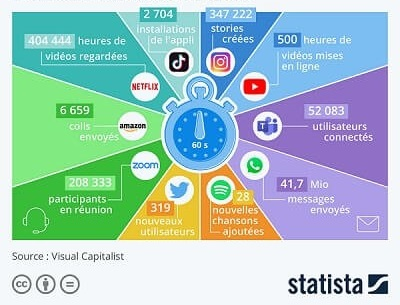
\includegraphics[scale=0.8]{img/fig1}
    \caption{1 minute d'Internet}
\end{figure}

En analysant la \textbf{figure 1.1} on constate l'énorme quantité de données qui circule.  En effet, durant cette minute sur internet alors que les utilisateurs de Facebook publient 147 000 photos, ceux d'Instagram partagent 347 222 stories et Twitter attire 319 nouveaux abonnés. Les plateformes de streaming ne sont pas en reste avec le SVOD Netflix notamment où les utilisateurs visionnent plus de 400 000 heures de vidéo en l'espace de 60 secondes et durant ce même laps de temps, 500 heures de vidéo sont publiées sur Youtube.
    \newpage
    \section{Définitions : }
\begin{center}
	\color[rgb]{0.2, 0.6, 0.2} Mais alors qu'est-ce que le Big Data ?
\end{center}

Plusieurs définitions peuvent être données au Big Data, étant un objet complexe polymorphe, sa définition varie. Parmi elles nous citons :

\begin{description}
	\item[Définition 1:]Le Big Data désigne l'ensemble des données numériques produites par l'utilisation des nouvelles technologies à des fins personnelles ou professionnelles. Cela regroupe les données d'entreprise ? Des contenus publiés sur le web, des transactions de commerce électronique, des échanges sur les réseaux sociaux, des données transmises par les objets connectés des données géolocalisées, ...etc.
	\item[Définition 2:]Le "Big Data" désigne les technologies et les initiatives qui impliquent des données trop diverses, en évolution rapide ou massives pour que les technologies, les compétences et les infrastructures conventionnelles puissent être traitées efficacement. Autrement dit, le volume, la vitesse ou la variété des données est trop important.
	\item[Définition 3:]Le terme Big Data fait référence aux données dont le coût de stockage, de gestion et d'analyse dans des systèmes de base de données traditionnels (relationnels et/ou monolithiques) serait généralement trop élevé. Habituellement, ces systèmes ne sont pas rentables, car ils ne disposent pas de la flexibilité nécessaire pour stocker des données non structurées (comme des images, du texte et des vidéos), pour accommoder des données "à haute vélocité" (en temps réel) ou pour s'adapter automatiquement à de très gros volumes de données (de l'ordre du pétaoctet).
\end{description}

\begin{figure}[h]
	\centering
	
\includegraphics[scale=0.6]{img/fig2}
	\caption{Le Big Data}
\end{figure}
    \newpage
    \section{Intérêts du Big-Data :}
Dans tous les secteurs, les entreprises utilisent le Big Data engrangé dans leurs systèmes à différentes fins. Il peut s'agir d'améliorer les opérations, de proposer un meilleur service client, de créer des campagnes marketing personnalisées basées sur les préférences des consommateurs, ou tout simplement d'augmenter le chiffre d'affaires.

Grâce au Big Data, les entreprises peuvent profiter d'un avantage compétitif face à leurs concurrents n'exploitant pas les données. Elles peuvent prendre des décisions plus rapides et plus précises, s'appuyant directement sur les informations.

\textit{Par exemple}, une entreprise peut analyser le Big Data pour découvrir de précieuses informations sur les besoins et les attentes de ses clients. Ces informations peuvent ensuite être exploitées pour créer de nouveaux produits ou des campagnes marketing ciblées afin d'accroître la fidélité client ou d'augmenter le taux de conversion. Une entreprise s'appuyant totalement sur les données pour aiguiller son évolution est qualifiée de ” data-driven ” (dirigée par les données).

\textit{\textbf{On peut citer comme exemple:} Netflix, en effet En 2015, la lettre envoyée par Netflix à ses actionnaires a démontré que la stratégie Big Data portait ses fruits. Au premier trimestre 2015, 4,9 millions de nouveaux abonnés ont été enregistrés, contre quatre millions à la même période en 2014. De même, 10 milliards d'heures de contenu ont été diffusées pendant ce trimestre. Grâce à une utilisation intelligente du Big Data, l'influence de Netflix ne cesse de s'accroître.}

En outre, le Big Data est utilisé dans le domaine de la recherche médicale. Il permet notamment d'identifier des facteurs de risque de maladies, ou de réaliser des diagnostics plus fiables et plus précis. Les données médicales permettent aussi d'anticiper et de suivre les éventuelles épidémies.

Les mégadonnées sont utilisées dans presque tous les secteurs sans exception. L'industrie de l'énergie s'en sert pour découvrir des zones de forage potentielles et surveiller leurs opérations ou le réseau électrique. Les services financiers l'utilisent pour gérer les risques et analyser les données du marché en temps réel.

Les fabricants et les entreprises de transport, quant à eux, gèrent leurs chaînes logistiques et optimisent leurs itinéraires de livraison grâce aux données. De même, les gouvernements exploitent le Big Data pour la prévention du crime ou pour les initiatives de Smart City.

pour résumer, Le Big Data permet de construire de meilleurs modèles, qui produisent
des résultats plus précis avec des approches extrêmement innovantes concernant
la manière dont :

\begin{itemize}[label=\textbullet]
	\item Les entreprises se commercialisent et vendent leurs produits.
	\item La gestion des ressources humaines.
	\item La réaction au catastrophes naturelles.
\end{itemize}

Ces exemples ne sont finalement qu'une poignée des opportunités qu'offre le Big Data. Les entreprises, et pas seulement, devront faire preuve d'imagination, d'organisation et d'un énorme sens d'analyse pour prendre la pleine mesure du phénomène. De cette maîtrise découle de nouveaux usages qui bouleverse notre façon de concevoir
Internet.



    \newpage
    \section{Les contraintes du Big Data :}

L'intérêt du Big Data, c'est de pouvoir tirer profit de nouvelles données produites par tous les acteurs (les entreprises, les particuliers, les scientifiques et les institutions publiques) dans le but d'optimiser son offre commerciale, ses services, développer la recherche et le développement mais aussi créer des emplois. Il y a certes des avantages mais aussi des inconvénients du Big Data.

Certaines publications discutent des obstacles au développement d'applications de méga données. Les principaux défis sont énumérés comme suit :

\begin{enumerate}[label=\protect\ding{\value*}, start=182]
\item \textbf{Représentation des données :} De nombreux ensembles de données présentent certains niveaux d'hétérogénéité dans le type, la structure, la sémantique, l'organisation, la granularité et l'accessibilité. La représentation des données vise à rendre les données plus significatives pour l'analyse informatique et l'interprétation des utilisateurs. Néanmoins, une représentation incorrecte des données réduira la valeur des données originales et peut même empêcher une analyse efficace des données.
\item \textbf{Réduction de la redondance et compression des données :} En général, il existe un niveau élevé de redondance dans les jeux de données. La réduction de la redondance et la compression des données sont efficaces pour réduire le coût indirect de l'ensemble du système en partant du principe que les valeurs potentielles des données ne sont pas affectées. Par exemple, la plupart des données générées par les réseaux de capteurs sont hautement redondantes.
\item \textbf{Gestion du cycle de vie des données :} Par rapport aux progrès relativement lents des systèmes de stockage, la détection et le calcul omniprésents génèrent des données à des taux et des échelles sans précédent. Nous sommes confrontés à de nombreux défis urgents, dont l'un est que le système de stockage actuel ne peut pas supporter des données aussi massives. De manière générale, les valeurs cachées dans le Big Data dépendent de la fraîcheur des données.
\item \textbf{Mécanisme analytique :} Le système analytique des méga données traitera des masses de données hétérogènes dans un temps limité. Cependant, les SGBDR traditionnels sont strictement conçus avec un manque d'évolutivité et d'extensibilité, ce qui ne pourrait pas répondre aux exigences de performance. Les bases de données non relationnelles ont montré leurs avantages uniques dans le traitement des données non structurées et ont commencé à se généraliser dans l'analyse des méga données. Même ainsi, il existe encore quelques problèmes de bases de données non relationnelles dans leurs performances et applications particulières. Des recherches supplémentaires sont nécessaires sur la base de données en mémoire et des échantillons de données basés sur une analyse approximative.
\item \textbf{Confidentialité des données :} La plupart des fournisseurs ou propriétaires de services de méga données ne pouvaient actuellement pas maintenir et analyser efficacement des ensembles de données aussi énormes en raison de leur capacité limitée. Ils doivent s'appuyer sur des professionnels ou des outils pour analyser ces données, ce qui augmente les risques potentiels pour la sécurité. Par exemple, l'ensemble de données transactionnelles comprend généralement un ensemble de données d'exploitation complètes pour piloter les processus métier clés. Ces données contiennent des détails et certaines informations sensibles telles que les numéros de carte de crédit.
\item \textbf{Gestion de l'énergie :} La consommation d'énergie des systèmes informatiques a beaucoup attiré l'attention du point de vue économique et environnemental. Avec l'augmentation du volume de données et des demandes analytiques, le traitement, le stockage et la transmission de données massives consommeront inévitablement de plus en plus d'énergie électrique.
\item \textbf{Expendabilité et évolutivité :} Le système analytique du Big Data doit prendre en charge les ensembles de données présents et futurs. L'algorithme analytique doit être capable de traiter des ensembles de données de plus en plus étendus et plus complexes.
\item \textbf{Coopération :} L'analyse du Big Data est une recherche interdisciplinaire, qui nécessite la coopération d'experts dans différents domaines pour exploiter le potentiel du Big Data. Une architecture de réseau Big Data complète doit être mise en place pour aider les scientifiques et les ingénieurs dans divers domaines à accéder à différents types de données et à utiliser pleinement leur expertise, afin de coopérer pour atteindre les objectifs analytiques.

\end{enumerate}


    \section{Caractéristiques des systèmes Big Data:}
Les méga-données sont un terme générique utilisé pour désigner toute collection de données volumineuse et complexe qui peuvent dépasser la capacité de traitement des systèmes et techniques de gestion de données conventionnels. Les applications du Big Data sont infinies. 

Les méga-données sont souvent caractérisées par le volume extrême des données, la grande variété de types de données et la vitesse à laquelle les données doivent être traitées. (Ces caractéristiques sont dites les 3V)
 
Ces caractéristiques ont été identifié pour la première fois par l'analyste Douglas Laney's membre du Gartner 10 dans un rapport publié en 2001. Plus récemment, plusieurs autres caractéristiques (autres V) ont été ajoutées aux descriptions des méga-données, notamment la véracité, la valeur et la variabilité. Bien que les méga-données ne correspondent à aucun volume de données spécifique, le terme est souvent utilisé pour décrire des téraoctets, des péta-octets et même des exa-octets de données capturées au fil du temps.

\begin{figure}[h]
	\centering
	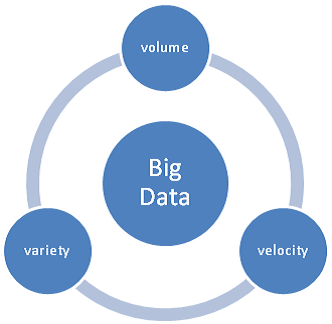
\includegraphics[scale=0.8]{img/fig3}
	\caption{Les 3 V.}
\end{figure}

Certaines personnes attribuent encore plus de V aux Big Data, les data scientiste et les consultants ont créé diverses listes contenant entre sept et 10 V.
On donne dans ce qui suit 10 caractéristiques "10V" sur les méga-données sachant que Les 3 premier critères basiques du Big Data sont le volume la vitesse ainsi que la variété :

\newcounter{compteur}
\stepcounter{compteur}
\subsection*{\arabic{compteur}. Le Volume:}
Le caractère volume est certainement celui qui est le mieux décrit par le terme Big de l'expression Big Data. Volume fait référence à la quantité d'informations, trop volumineuse pour être acquise, stockée, traitée, analysée et diffusée par des outils standards. Ce caractère peut s'interpréter comme le traitement d'objets informationnels de grande taille ou de grandes collections d'objets.

\textit{\textbf{Exemple :} les utilisateurs d'Instagram partagent 347 222 stories en 60secondes.}

\stepcounter{compteur}
\subsection*{\arabic{compteur}. La Variété:}
Elle fait référence aux différentes formes toujours croissantes que les données peuvent prendre, en effet les données Big Data ne sont pas seulement des nombres, des dates et des chaînes. Les méga-données englobent également une grande variété de types de données, y compris des données structurées dans des bases de données SQL et des entrepôts de données, des données non structurées, telles que des fichiers texte et document conservés dans des clusters Hadoop ou des systèmes NoSQL, et des données semi-structurées, telles que des journaux de serveur Web ou la diffusion des données à partir de capteurs.

\textit{\textbf{Exemple :} Un projet d'analyse des méga-données peut tenter d'évaluer le succès d'un produit et les ventes futures en corrélant les données de ventes passées, les données de retour et les données de révision des acheteurs en ligne pour ce produit.}

\stepcounter{compteur}
\subsection*{\arabic{compteur}. La vélocité:}
Dernière dimension, tout aussi importante que les précédentes, la vélocité traduit la capacité à produire rapidement les données et à les transformer en temps utile pour leurs utilisateurs. L'exercice, déjà difficile dans un contexte "classique", prend toute sa valeur lorsqu'il doit être applique à d'immenses volumes de données de toutes sortes.

\textit{\textbf{Exemple :} Google traite en moyenne plus de "40 000 requetés de recherche par seconde", ce qui représente environ 3,5 milliards de recherches par jour.}

\stepcounter{compteur}
\subsection*{\arabic{compteur}. La Véracité:}
Elle fait référence aux biais, au bruit et aux anomalies dans les données. Ou, mieux encore, il fait référence aux incertitudes et à la fiabilité des données souvent incommensurables.

\textit{\textbf{Exemple :} Dans le cadre d'un sondage réalisé par IBM, 27\% des entreprises interrogées avouent ne pas être certaines de l'exactitude des données qu'elles collectent. De même, un chef d'entreprise sur trois utilise les données pour prendre des décisions, mais n'a pas vraiment confiance. Ce manque de véracité et de qualité des données coûte environ 3,1 trillions de dollars par an aux États-Unis.}

\stepcounter{compteur}
\subsection*{\arabic{compteur}. La Valeur:}
Toutes les données collectées n'ont pas une valeur commerciale réelle et l'utilisation de données inexactes peut affaiblir les informations fournies par les applications d'analyse. Il est essentiel que les organisations utilisent des pratiques telles que le nettoyage des données et confirment que les données sont liées à des problèmes commerciaux pertinents avant de les utiliser dans un projet d'analyse de Big Data. 

On peut dire que les autres caractéristiques du Big Data n'ont pas de sens si on ne tire pas de valeur commerciale de ces données. Les Données massives offrent une valeur substantielle : comprendre mieux les clients. Les cibler en conséquence, optimiser les processus et améliorer les performances de la machine ou de l'entreprise. Avant de se lancer dans une stratégie Big Data, on doit comprendre le potentiel et les caractéristiques les plus difficiles.

\textit{\textbf{Exemple :} La mise en place d'une analyse Big Data a permis à la société de développement d'éoliennes Vestas 11 d'optimiser son processus d'identification des meilleurs emplacements pour implanter ses éoliennes. Le traitement Big Data a engendré une augmentation de la performance de production d'électricité et une réduction des coûts énergétiques associés.}

\textbf{Remarque :} Certaines personnes attribuent encore plus de V aux Big Data ; les scientifiques des données et les consultants ont créé d'autres listes en ajoutant la variabilité, la validité, la visualisation, la volatilité ainsi que la vulnérabilité.

\stepcounter{compteur}
\subsection*{\arabic{compteur}. La Variabilité:}
La variabilité dans le Big Data fait référence à plusieurs sens. Dans un premier temps elle désigne le nombre d'incohérences dans les données. Celles-ci doivent être détectées par des techniques de détection d'anomalies et de valeurs aberrantes pour faciliter la création d'analyse significative. 

Les méga-données sont également variables en raison de la diversité de dimensions résultant de multiples types et sources de données. La variabilité peut également faire référence à la vitesse incohérente à laquelle les données volumineuses sont chargées dans la base de données.

\textit{\textbf{Exemple :} L'équipe d'IBM 12 fait participer Watson 13 au célèbre jeu télévisé américain Jeopardy, un jeu ou les candidats doivent trouver les réponses à des questions posées. Watson devait "être capable de comprendre l'énoncé des questions, buzzer pour prendre la main, disséquer une réponse dans son sens pour déterminer quelle était la bonne question". Les mots n'ont pas de définitions statiques et leur signification peut varier énormément dans le contexte.}

\stepcounter{compteur}
\subsection*{\arabic{compteur}. La Validité:}
Similaire à la véracité, la validité fait référence à la précision et à la correction des données pour l'usage auquel elles sont destinées. Selon Forbes 14, environ 60\% du temps d'un scientifique est consacré au nettoyage de ses données avant de pouvoir effectuer une analyse. L'avantage de l'analyse des données massives est aussi primordial que celui des données sous-jacentes. On doit donc avoir de bonnes pratiques de gouvernance des données pour garantir une qualité des données cohérente, des définitions communes et des métadonnées.

\textit{\textbf{Exemple :} La date d'une transaction est  02/07/1994 alors que l'activité de la société a débuté en 2000.}

\stepcounter{compteur}
\subsection*{\arabic{compteur}. La Volatilité:}
On se pose les questions :\textit{‘quel âge doivent avoir les données pour qu'elles soient considérées comme non pertinentes, historiques ou obsolète ?’,  ‘Combien de temps faut-il conserver les données ?’} Avant l'ère du Big Data, en général, on stockait les données indéfiniment. Quelques téraoctets de données ne pouvaient pas engendrer de dépenses de stockage élevées. 

En raison de la vitesse et du volume de ces données massives, leur volatilité doit être soigneusement prise en compte. Il est maintenant fondamental d'établir des règles pour la disponibilité et à la mise à jour des données a de garantir une récupération rapide des informations en cas de besoin.

\textit{\textbf{Exemple :} Une entreprise e-commerce peut ne pas souhaiter conserver un historique des achats client d'un an. Parce qu'après un an la garantie par défaut sur leur produit expire, il n'y a donc aucune possibilité de restaurer ces données.}

\stepcounter{compteur}
\subsection*{\arabic{compteur}. La Visualisation:}
Une autre caractéristique du Big Data est la difficulté à les visualiser. Les logiciels de visualisation de données volumineuses actuels sont confrontés à des problèmes techniques en raison des limitations de la technologie en mémoire, de leur faible évolutivité, de leur fonctionnalité et de leur temps de réponse. Il est impossible de se fier aux graphiques traditionnels lorsqu'on essaye de tracer un milliard de points de données. Il est donc nécessaire d'avoir différentes manières de représenter des données. Telles que la mise en cluster de données ou l'utilisation de cartes d'arbres, de sunbursts, de coordonnées parallèles, de diagrammes de réseau circulaires ou de cônes. 

Si on associe cela avec la multitude de composante résultant de la variété et de la vélocité des données massives et des relations complexes qui les lient, il est possible de voir qu'il n'est pas si simple de créer une visualisation significative.

\textit{\textbf{Prenons l'exemple :} du tableau suivant qui fait apparaître deux séries de chiffres : le chiffre d'affaires en France et le chiffre d'affaires du reste du monde. La lecture de ce tableau et sa signification ne sont pas immédiates.}

\begin{figure}[h]
	\centering
	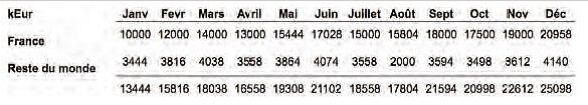
\includegraphics[scale=0.8]{img/fig5}
	\caption{Évolution du chiffre d'affaires par région.}
\end{figure}

\textit{Mais si nous représentons les séries de chiffres sous forme graphique (ci-dessous), on comprend en un coup d'œil que le chiffre d'affaires en France progresse et que le chiffre d'affaires du Reste du monde stagne.}

\begin{figure}[h]
	\centering
	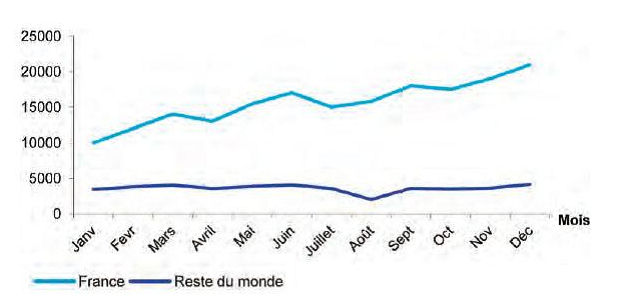
\includegraphics[scale=0.8]{img/fig6}
	\caption{Évolution du chiffre d'affaires par région.}
\end{figure}

\stepcounter{compteur}
\subsection*{\arabic{compteur}. La Vulnérabilité:}
Le Big Data apporte de nouveaux problèmes de sécurité. Malheureusement, il y a quotidiennement des violations de données massives.

\textit{\textbf{Exemple :} Rapporté par CRN15 : en mai 2016, un pirate informatique appelé Peace a posté des données sur le dark web pour les vendre, qui auraient inclus des informations sur 167 millions de comptes LinkedIn et 360 millions d'e-mails et de mots de passe pour les utilisateurs de MySpace 16.}

\begin{figure}[h]
	\centering
	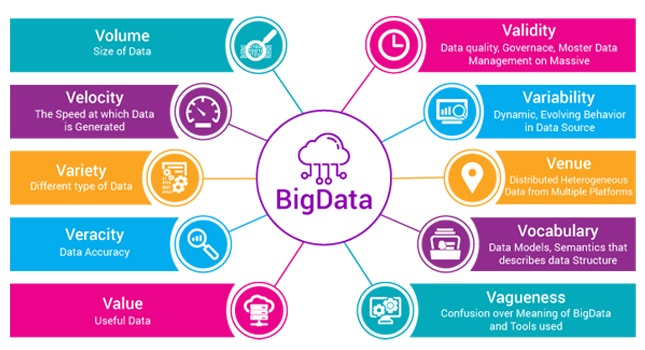
\includegraphics[scale=0.5]{img/fig4}
	\caption{Les 10 V.}
\end{figure}

\textbf{Remarque :} Il existe d'autres sources qui parlent de 54 Vs pour les caractéristiques du Big Data tel que la venue (le lieu), valence, vocabulaire, imprécision...etc.







    
    \section{Choses qui viennent du Big Data (Exemples du Big Data):}
Le concept de big data est une gestion groupée de différentes formes de données générées par divers appareils (Android, iOS, etc.), d'applications (applications musicales, applications Web, applications de jeux, etc.) ou d'actions (recherche par SE, navigation à travers des types similaires de pages Web, etc.). Voici la liste de certains champs de données couramment trouvés qui sont sous l'égide du Big Data:

\begin{description}
\item[Données sur les boîtes noires :]
Les données des boîtes noires sont un type de données recueillies à partir d'hélicoptères, d'avions et de jets privés et gouvernementaux. Ces données comprennent la capture des sons de l'équipage de conduite, l'enregistrement séparé du microphone ainsi que des écouteurs, etc.
\item[Données boursières :]
Les données boursières comprennent diverses données préparées sur « l'achat » et la « vente » de différentes décisions brutes et bien prises.
\item[Données sur les médias sociaux :] 
Ce type de données contient des informations sur les activités des médias sociaux qui incluent des messages soumis par des millions de personnes dans le monde entier.
\item[Données sur les transports :] 
Les données sur les transports comprennent les modèles de véhicules, la capacité, la distance (d'une source à l'autre) et la disponibilité de différents véhicules.
\item[Données des moteurs de recherche :] 
récupérez une grande variété d'informations non traitées stockées dans les bases de données SE.

\end{description}
    \newpage
    \section{Les sources du Big Data :}
Pour réussir avec le Big Data, il est important que les entreprises disposent du savoir-faire pour passer en revue les différentes sources de données disponibles et classer en conséquence leur convivialité et leur pertinence. Deux classifications des sources du Big Data sont données dans ce qui suit :

\begin{enumerate}
\item Selon qu'elles soient internes ou externe à l'entreprise.
\item Selon leur provenance.
\end{enumerate}

\subsection{Les données internes ou externes à l'entreprise}
Les données sont internes si une entreprise les génère, les possède et les contrôle.

\textbf{Exemple :}
\begin{itemize}[label=\textbullet]
\item Module ERP d'entreprise.
\item Capteurs, contrôleurs.
\item Centres d'appels internes.
\item Journaux de site Web.
\end{itemize}

Les données externes sont des données publiques ou des données générées en dehors de l'entreprise ; en conséquence, la société ne la possède ni ne la contrôle. Exemple :
\begin{itemize}[label=\textbullet]
\item Médias sociaux.
\item Statistiques officielles.
\item Ensembles de données accessibles au public pour l'apprentissage automatique.
\end{itemize}

\subsection{Les sources du Big Data selon leur provenances :}
Les données les plus volumineuses sont utilisées aujourd'hui par les organisations et les entreprises dans le seul but d'effectuer des analyses. Toutefois, avant de pouvoir extraire des informations et des renseignements précieux à partir de données importantes, ces dernières doivent connaître plusieurs sources de données importantes. Les données, comme nous le savons, sont massives et existent sous diverses formes. Si elles ne sont pas bien classées ou si elles ne proviennent pas d'une source sure, elles peuvent finir par faire perdre du temps et des ressources précieuses. Afin de réussir avec les données volumineuses, il est important que les entreprises aient le savoir-faire nécessaire pour faire le tri entre les différentes sources de données disponibles et classer en conséquence leur utilité et leur pertinence.

\begin{figure}[h]
	\centering
    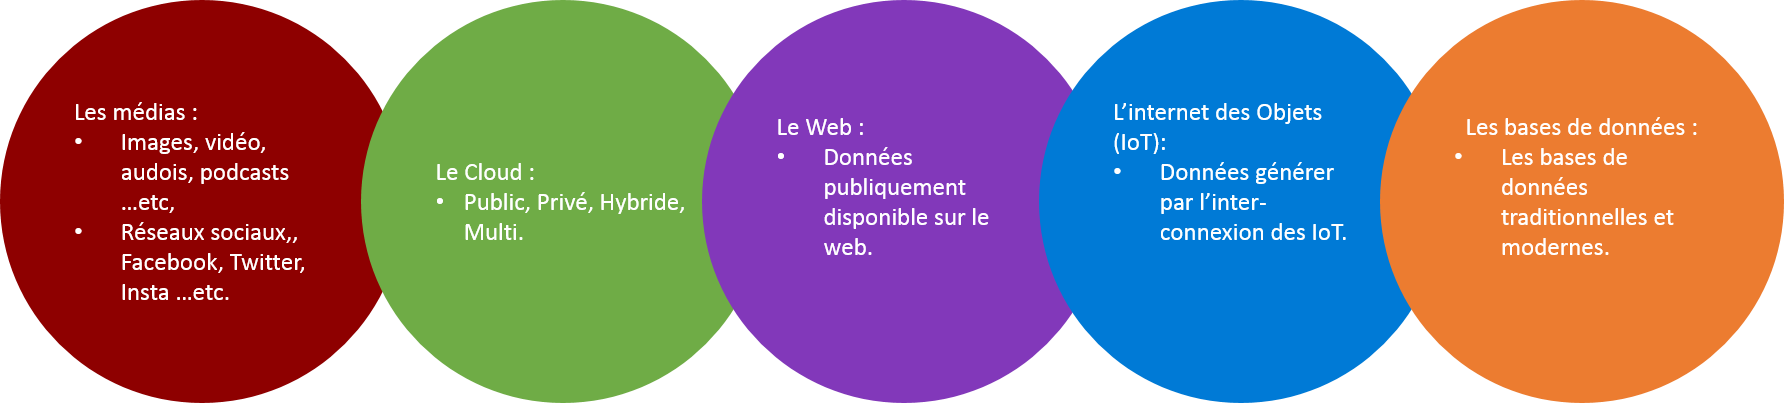
\includegraphics[scale=0.5]{img/fig11}
    \caption{Les sources du Big Data}
\end{figure}

\subsubsection{Les médias :}
Les médias sont la source la plus populaire de méga données, car ils fournissent des informations précieuses sur les préférences des consommateurs et l'évolution des tendances. Ces données sociales proviennent des mentions J'aime, des tweets et des retweets, des commentaires, des téléchargements de vidéos et des médias généraux qui sont téléchargés et partagés via les plateformes de médias sociaux préférées au monde. Ce type de données fournit des informations inestimables sur le comportement et le sentiment des consommateurs et peut être extrêmement influent dans les analyses marketing.

\textit{\textbf{Exemple :}Les médias comprennent les médias sociaux et les plates-formes interactives, telles que Google, Facebook, Twitter, YouTube, Instagram, ainsi que des supports génériques tels que des images, des vidéos, des audio et des podcasts qui fournissent des informations sur l'interaction utilisateur.}

\subsubsection{Le Cloud :}
Aujourd'hui, avec la croissance accélérée du volume de données utilisé par les applications, de nombreuses organisations ont déplacé leurs données vers des serveurs Cloud pour fournir des services évolutifs,  ables et hautement disponibles [12].

Le stockage Cloud héberge des données structurées et non structurées et fournit aux entreprises des informations en temps réel et des informations à la demande. Le principal attribut du Cloud computing est sa flexibilité et son évolutivité. Comme les méga données peuvent être stockées et sourcées sur des Clouds publics ou privés, via des réseaux et des serveurs, le Cloud constitue une source de données efficace et économique car les ressources sont fournis à la demande et on ne paye que les ressources utilisées.

\subsubsection{Le Web :}
Le Web public constitue une source répandu et facilement accessible pour le Big Data. Les données sur le Web ou “Internet“ sont généralement disponibles pour les particuliers et les entreprises. De plus, des services Web tels que Wikipédia fournissent des informations gratuites et rapides à tout le monde. Le Web public est également une autre bonne source de données sociales, et des outils comme Google Trends peuvent être utilisés à bon escient pour augmenter le volume de données.

L'énormité du Web garantit sa polyvalence et est particulièrement bénéfique pour les start-ups et les PME, car elles n'ont pas à attendre pour développer leur propre infrastructure et référentiels de Big Data avant de pouvoir tirer parti du Big Data.

\subsubsection{L'Internet Des Objets (IoT) :}
Les données machine sont définies comme des informations générées par des équipements industriels, des capteurs installés dans des machines et même des journaux Web qui suivent le comportement de l'utilisateur. En logistique, il peut s'agir de capteurs qui servent à la traçabilité des biens pour la gestion des stocks et les acheminements.

En domotique, l'IoT recouvre tous les appareils électroménagers communicants, les capteurs, les compteurs intelligents et systèmes de sécurité connectés des appareils de type box domotique. Le phénomène IoT est également très visible dans le domaine de la santé et du bien-être avec le développement des montres connectées, des bracelets connectés et d'autres capteurs surveillant des constantes vitales.

\textit{\textbf{Exemple :} En Tennis, la marque Zepp propose un système de capteur connecté qui analyse vos performances sur le terrain. Il suffit de fixer le capteur sur le manche de n'importe quelle raquette de tennis et de se mouvoir pour obtenir un retour d'information instantané sur iPhone, iPad ou appareil Android.}

\subsubsection{Les bases de données :}
Les entreprises préfèrent aujourd'hui utiliser une fusion de bases de données traditionnelles et modernes pour acquérir des méga données pertinentes. Cela permet d'ouvrir la voie à un modèle de données hybride avec un faible coût d'investissement. De plus, ces bases de données sont également déployées à plusieurs  ns de Business Intelligence. Le processus d'extraction et d'analyse de données parmi de vastes sources de méga données est un processus complexe qui peut être frustrant. Ces complications peuvent être résolues si les organisations englobent toutes les considérations nécessaires des méga données, et prennent en compte les sources de données pertinentes et les déploient d'une manière bien adaptée à leurs objectifs organisationnels.

\textit{\textbf{Exemple :} Les bases de données les plus populaires Microsoft SQL Server, MongoDB, Oracle, MySQL et IBM Db2 ...etc.}


    \newpage
    \section{Les métiers du Big Data:}
Le marché du big data est à l'origine d'un nombre croissant de métiers Les entreprises de tous les secteurs cherchent désormais à exploiter les données à leur disposition pour aiguiller leur stratégie et leur développement. Toutefois, pour être en mesure d'exploiter ces données, les entreprises doivent s'appuyer sur des compétences et du savoir-faire de professionnels hautement qualifiés capables d'utiliser les technologies analytiques. Ainsi, le Big Data a donné naissance à de nombreux nouveaux métiers : 

\newcounter{compteurM}
\stepcounter{compteurM}
\subsection*{\arabic{compteurM}. LE CHIEF DATA OFFICER}
Le chief data officer se charge de gouverner la data, qui constitue un capital vital pour l'entreprise. Il a pour mission de trier les masses de données disponibles afin de faciliter l'accès à l'information pertinente permettant des prises de décision adaptées. Pour ce faire, il doit constamment vérifier la fiabilité des informations recueillies et s'appuyer sur des éléments objectifs provenant de données statistiques. Le chief data officer intervient dans la construction et la mise en application d'une stratégie de gouvernance des données et travaille en collaboration avec d'autres professionnels tels que les data scientists, les spécialistes en business intelligence et les statisticiens.

\stepcounter{compteurM}
\subsection*{\arabic{compteurM}. LE DATA ENGINEER}
Le data engineer (ou ingénieur de données) est un professionnel spécialisé dans la gestion des données. Sa mission principale consiste à recueillir, croiser, trier et réaliser des opérations de nettoyage des données. Il doit aussi gérer leur stockage dans différentes bases de données et exploiter des masses d'information sous divers formats.

\stepcounter{compteurM}
\subsection*{\arabic{compteurM}. LE DATA SCIENTIST}
Le data scientist, appelé également analyste en big data, est un spécialiste de l'analyse des données massives. Sa mission prend effet après celle de l'ingénieur de données : le data engineer intervient dans la gestion des données alors que le data scientist assure le traitement de ces données pour en extraire de la valeur. Pour ce faire, le data scientist se charge de développer des algorithmes statistiques afin de tirer des informations pertinentes permettant de classifier des données, d'anticiper un comportement ou encore de préconiser des actions appropriées. Il doit donc avoir de solides connaissances en informatique, en statistiques et en management. Le data scientist doit également maîtriser les techniques du datamining et les outils de traitement des bases de données tels que Hadoop, MapReduce, Java, BigTable et NoSQL.

Les analystes en big data interviennent dans divers domaines d’activité : ils développent dans l’e-commerce et les réseaux sociaux les algorithmes de recommandation de pages, de profils et de produits

\stepcounter{compteurM}
\subsection*{\arabic{compteurM}. L’ARCHITECTE BIG DATA}
Data architect en anglais, l'architecte big data a pour mission principale d'organiser des données brutes. C'est un métier plus conceptuel que technique, qui assure la création des infrastructures de stockage et conçoit des solutions de gestion des données massives. Il propose également aux décideurs la cartographie des outils Hadoop à mettre en place. L'architecte big data travaille en étroite collaboration avec le data scientist, tout en lui fournissant les données brutes à traiter. Il intervient également dans l'étude de la faisabilité technique et la mise en place des outils et la configuration des machines.

\stepcounter{compteurM}
\subsection*{\arabic{compteurM}. LE DÉVELOPPEUR BIG DATA}
Le développeur big data maîtrise les différents langages informatiques notamment Java et Python. Il assure la cohérence du système, la gestion des pannes et garantit la continuité du service. Les données massives sont en effet au centre des préoccupations du métier de développeur big data. Ce profil travaille aussi en collaboration avec le data scientist : alors que ce dernier intervient dans la conception des algorithmes facilitant la prise de décision, le développeur big data assure leur mise en marche. Il fait partie des rares profils du big data à pouvoir gérer toutes les catégories des outils d'Hadoop pour des objectifs d'évaluation.

\stepcounter{compteurM}
\subsection*{\arabic{compteurM}. LE GROWTH HACKER}
Le growth hacker n'est pas simplement un métier, c'est surtout un état d'esprit qui permet de développer plusieurs techniques webmarketing. C'est un profil à la croisée du marketing, du développement logiciel et du big data, qui a pour mission d'accélérer la croissance d'un produit ou d'un service propre à la structure qui l'embauche. Il utilise pour cela des solutions digitales innovantes et des pratiques de pointe afin d'accroître le revenu de son entreprise. Pour ce faire, le growth hacker cherche à développer, à partir d'Hadoop, de nouveaux produits et de nouvelles fonctionnalités. Il utilise également les outils de base de données (SQL) et les langages d'abstraction. De plus, comme tous les professionnels du marketing, il est en recherche constante de clients. Le growth hacker est très prisé par les start-up et les entreprises qui souhaitent se réinventer constamment. 

\stepcounter{compteurM}
\subsection*{\arabic{compteurM}. LE DATA MINER}
Le data miner assure la transmission des connaissances utiles à la progression de l'entreprise. Il dégage ainsi les tendances relatives à la consommation des clients pour en sortir avec une stratégie marketing réalisable sur le terrain. Pour se positionner sur le marché, il prend en compte les habitudes de consommation et les tarifs appliqués par la concurrence. De plus, il assure le tri des informations potentiellement exploitables, analyse les données après les avoir formatées et nettoyées. Il réalise aussi des rapports d'analyse, des tableaux de visualisation des données et compare les performances de l'entreprise pour les ajuster aux objectifs et prévisions. Le data miner a de grandes capacités d'observation et d'analyse de données.

\stepcounter{compteurM}
\subsection*{\arabic{compteurM}. L'ADMINISTRATEUR BIG DATA}
L'administrateur joue un rôle primordial dans la structure informatique d'une entreprise. Il intervient dans la conception, l'optimisation et la configuration des infrastructures de stockage des données massives. Il assure également la sécurisation des données ainsi que l'attribution des autorisations et des droits d'accès aux différents utilisateurs. L'administrateur big data maîtrise les langages de programmation, les outils d'administration Hadoop et les protocoles de sécurité. Il vérifie la disponibilité de l'information à tout moment et apporte les modifications nécessaires sur les bases de données.
    \newpage
    \section{Les technologies du Big Data:}
Cette technologie est importante pour présenter une analyse plus précise qui conduit l’analyste d’affaires à prendre des décisions très précises, assurant ainsi une efficacité opérationnelle plus considérable en réduisant les coûts et les risques commerciaux. Maintenant, pour implémenter de telles analyses et détenir une telle variété de données, il faut avoir besoin d’une infrastructure qui puisse faciliter et gérer et traiter d’énormes volumes de données en temps réel. De cette façon, le Big Data est classé en deux sous-catégories, le Big Data opérationnel qui comprend des données sur des systèmes et le Big Data analytique qui comprend des systèmes. 

Nous décrivons ensuite ici tous les composants qui font partie des solutions Big Data sous de nombreux angles : matériel, méthodologies, logiciels et applications de base, etc.

Pour mieux catégoriser ces concepts, nous les avons a répartis en différentes sections selon l'objectif visé par chacun. Ces catégories sont : l'infrastructure, le stockage, le traitement et les composants de haut niveau.

\subsection{Les infrastructures :}
Le développement du Big Data commence avec les clusters Big Data qui exécutent en parallèle les instructions d'un logiciel de haut niveau. Le cluster est artitionné en deux types de nœuds selon la fonction principale exercée:

\begin{itemize}[label=\textbullet]
	\item Nœuds de données ou esclaves (informatique).
	\item Nœuds de gestion ou maîtres (gestion).
\end{itemize}

Outre leur fonction, le maître et les esclaves peuvent être différenciés par leurs capacités de calcul et leur quantité dans le champ de nœuds.

Les esclaves sont chargés de surveiller les données partitionnées, de traiter et d'interroger les données locales. Les unités de données et de traitement doivent être aussi proches que possible pour éviter les retards introduits par les mouvements entre les partitions. Les nœuds de données sont gourmands en disque et standard en termes de capacités de calcul et de mémoire.

Les maîtres reçoivent et transforment les programmes des applications clientes en instructions parallèles qui peuvent être comprises par les esclaves. Une fois que les applications clientes ont atteint le démon maître, elles finissent par démarrer ou réveiller plusieurs processus dans les esclaves qui retournent finalement une sortie suivant la direction opposée. Parmi l'ensemble des responsabilités approuvées pour les nœuds de gestion figurent :

\begin{itemize}[label=\textbullet]
	\item La récupération après défaillance.
	\item La gestion des ressources.
	\item La planification des travaux.
	\item La surveillance ou la sécurité.
\end{itemize}

Pour accomplir ces tâches, les maîtres nécessitent une puissance de calcul et de mémoire élevée. Dans les clusters Big Data standard, il suffit de garder deux maîtres supports qui se surveillent mutuellement.

Les deux types de nœuds sont connectés via une connexion réseau, généralement LAN (Ethernet ou InfiniBand). Certaines configurations permettent également de connecter les maîtres de déférents centres de données sur un réseau WAN pour éviter facilement les défaillances du système. Dans chaque centre de données, le maître et les esclaves sont interconnectés en privé pour ingérer des données, déplacer des données entre les nœuds et effectuer des requêtes. Il existe également un autre réseau public qui sert de façade entre le client et le service de gestion (SSH, VNC, interface web,..)

\subsection{Les technologies de traitements :}

\begin{figure}[h]
	\centering
	
\includegraphics[scale=0.4]{img/part1/1.8}
	\caption{Hadoop.}
\end{figure}

Dans cette section nous parlerons de l'arrivée des technologies de traitement ajustées, plus spécialement sur la mise au point de modes de calcul à haute performance ( MapReduce ), nous parlerons de ( Hadoop ) une solution de Big Data très largement utilisée pour effectuer des analyses sur de très grands nombres de données.

\begin{enumerate}[label=\protect\ding{\value*}, start=182,font=\color{blue}]
\item \subsubsection{Map-reduce :}
MapReduce a été introduit par Google et décrit en détails dans la publication « MapReduce : Simplified Data Processing on Large Clusters » publiée en 2004 et ça pour faciliter la mise en œuvre de ses workfows de traitement parallèle. L'objectif principal était de remplacer la programmation complexe et non intuitive sur l'informatique distribuée (préalablement abordée par les plateformes HPC) par une plateforme transparente moderne avec seulement deux fonctions : Map et Reduce. Ces deux fonctions définies par l'utilisateur permettent aux utilisateurs d'utiliser les ressources distribuées sans se plaindre du réseau, de la planification, de la récupération après défaillance, etc.

Un modèle aussi intuitif que le MapReduce ne nécessite pas d'expertise concernant le parallélisme et les systèmes distribués. Son Framework Plug-and-Play embarque tous les détails pour implémenter les systèmes de calcul parallèle, la persistance et la résilience, l'optimisation et l'équilibre des ressources.

\begin{itemize}[label=\ding{51}]
\item \textbf{Principe de MapReduce :}
MapReduce applique le principe dit « diviser pour distribuer pour régner », la stratégie mise en place pour exécuter un calcul sur des données massives consiste a : 
\begin{itemize}[label=\textbullet]
\item \textbf{Découper} les données en sous ensemble de plus petite taille, appelés lors ou fragments.
\item \textbf{Affecter} chaque lot a une machine permettant ainsi leur traitement en parallèle.
\item \textbf{Agréger} l'ensemble des résultats intermédiaires obtenu pour chaque lot pour construire le résultat final.
\end{itemize}
\newpage
Ce dernier se repose sur deux fonctions : Map qui permet aux différents points du cluster distribué de distribuer leur travail. La fonction Reduce qui permet de réduire la forme finale des résultats des clusters en un seul résultat.

Le rôle du développeur d’applications distribuées c’est de réfléchir en MapReduce :
\begin{itemize}[label=\textbullet]
\item Choisir une manière de découper les données afin que l’opération MAP soit parallèlisable. 
\item Choisir la clé a utilisé pour le problème ciblé.
\item Ecrire le code de la fonction pour l’opération MAP.
\item Ecrire le code de la fonction pour l’opération REDUCE.

\end{itemize}
\subparagraph{Exemple d'utilisation de MapReduce:}
\textit{Nous allons tester un programme MapReduce grâce à un exemple très simple, le WordCount, l'équivalent du HelloWorld pour les applications de traitement de données. Le Wordcount permet de calculer le nombre de mots dans un fichier donné, en décomposant le calcul en deux étapes:
L'étape de Mapping, qui permet de découper le texte en mots et de délivrer en sortie un flux textuel, où chaque ligne contient le mot trouvé, suivi de la valeur 1(pour dire que le mot a été trouvé une fois)
et l'étape de Reducing, qui permet de faire la somme des 1 pour chaque mot, pour trouver le nombre total d'occurrences de ce mot dans le texte.}

\begin{figure}[h]
	\centering
	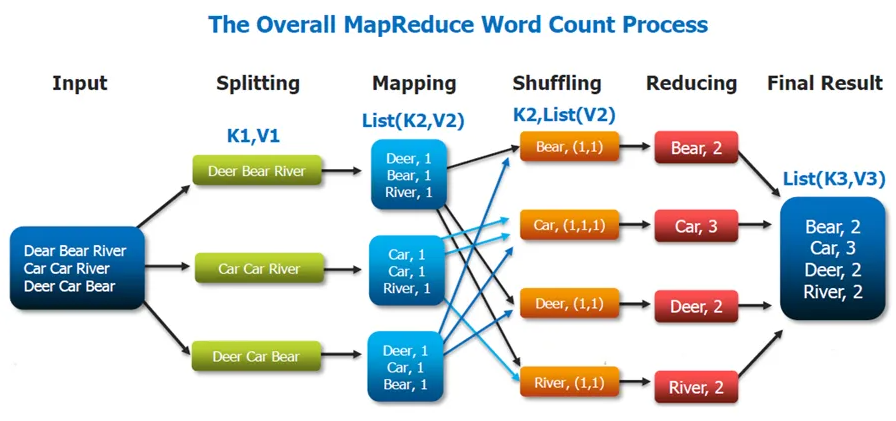
\includegraphics[scale=0.6]{img/part1/1.9}
	\caption{Exemple de Word Count.}
\end{figure}

\item \textbf{Les avantages de MapReduce: }Parmi les avantages de la programmation MapReduce nous citons
\begin{itemize}[label=\textbullet]
	\item La scalabilité.
	\item La flexibilité.
	\item La sécurité et l'authentification.
	\item Le traitement parallèle.
	\item La disponibilité.
	\item Un modèle simple de programmation.
\end{itemize}

\end{itemize}

\item \subsubsection{HADOOP:}
MapReduce a tout son intérêt dans le Big Data car il permet le passage à l’échelle des traitements sur de gros volumes de données, cependant il faut une infrastructure logiciel dédiée qui permettent d’exécuté le schéma MapReuce de manière distribué sur les clusters machine. C’est là qu’intervient Hadoop.

Hadoop est un framework logiciel open source permettant de stocker des données, et de lancer des applications sur des grappes (cluster) de machines standards. Cette solution offre un espace de stockage massif pour tous les types de données, une immense puissance de traitement et la possibilité de prendre en charge une quantité de tâches virtuellement illimitée. Basé sur Java, ce framework fait partie du projet Apache, sponsorisé par Apache Software Foundation.

Grâce a MapReduce, il permet de traiter les immenses quantités de données. Plutôt que de devoir déplacer les données vers un réseau pour procéder au traitement, MapReduce permet de déplacer directement le logiciel de traitement vers les données. 

Hadoop se compose essentiellement de :

\begin{figure}[h]
	\centering
	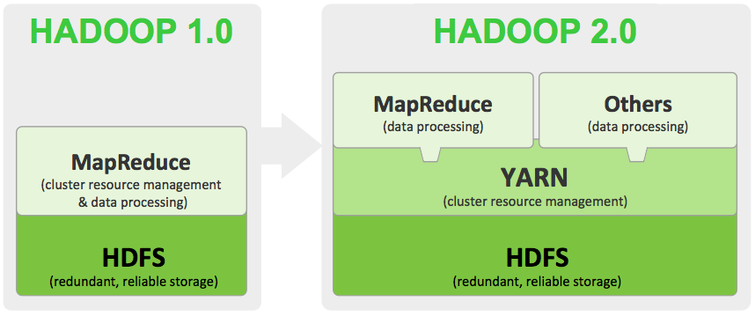
\includegraphics[scale=0.4]{img/part1/1.10}
	\caption{Les composants d'Hadoop.}
\end{figure}

\begin{itemize}[label=\ding{51}]
\item \textbf{Système de gestion de fichiers HDFS (Hadoop Distributed File System) :} HDFS est un système de fichiers distribué, extensible et portable Inspiré par GFS et écrit en Java. Il est conçu pour être un système de stockage distribué, évolutif et résilient, conçu pour interagir facilement avec MapReduce. Il fournit une bande passante d'agrégation importante tout au long du réseau. Comme pour GFS, un réseau HDFS est composé d'un nœud maître appelé Namenode et des serveurs de données appelés Datanodes, de grande taille par défaut 64 Mo pour optimiser les temps de transfert et d'accès. Il est toutefois possible de monter à 128 Mo, 256 Mo, 512 Mo voire 1 Go.
\item \textbf{Modèle de programmation Map-reduce :} Le framework MapReduce permet de traiter les immenses quantités de données. Plutôt que de devoir déplacer les données vers un réseau pour procéder au traitement, MapReduce permet de déplacer directement le logiciel de traitement vers les données. Ce modèle fera l'objet de la deuxième technologie que nous allons présenter.
\item \textbf{YARN (Yet Another Ressource Negiciator)}à été ajoutée comme une fonctionnalité clé depuis Hadoop 2.0 déployée en 2013, Avant son ajout, Hadoop ne pouvait exécuter que des applications MapReduce. YARN a donc beaucoup augmenté les cas d’usage potentiels du framework. En découplant la gestion des ressources et la planification du composant de traitement de données de MapReduce, YARN a également permis à Hadoop de prendre en charge davantage d’applications et de types de traitement différents.

\end{itemize}

Hadoop 3 sortie le 13 décembre 2017 apporte son lot de nouveautés qu’il convient de présenter:
\begin{itemize}[label=\textbullet]
\item La première différence provient de la gestion des conteneurs. La troisième apporte davantage d’agilité grâce à l’isolation des paquets de Docker.
\item Le coût d’utilisation d’Hadoop 3 est également plus faible. La deuxième version demande plus d’espace de stockage. Là où la troisième version demande 9 blocs de  stockage.
\item Autre différence majeure, Hadoop 2 ne gère qu’un seul namenode. Cet outil de gestion de l’arborescence du système de fichiers, les métadonnées des fichiers et les répertoires. La version suivante peut en gérer plusieurs, ce qui permet d’augmenter de manière exponentielle la taille des infrastructures.
\item Enfin, cette dernière version du système HDFS ouvre de nouvelles perspectives pour les concepteurs d’algorithmes de machine learning et de deep learning. 
\end{itemize}

\item \subsubsection{Les bases de données NoSQL :}
De nos jours, l'ubiquité de la connexion Internet est une réalité (les voitures que nous conduisons, les montres que nous portons, nos petits appareils médicaux domestiques, nos réfrigérateurs et congélateurs, nos Smartphones et ordinateurs portables). De plus, les données numériques produites par les êtres humains, dont les séquences vidéo, les photos et autres, atteignent des volumes importants de plusieurs EO par jour. Ces données actuellement stockées dans des bases qui leur ont été conçues spécifiquement sont gérés par des logiciels de gestion de bases de données volumineuses, jouant le rôle d'intermédiaires entre les bases de données d'un côté et les applicatifs et leurs utilisateurs de l'autre. On parle ici des bases de données non-relationnelles, dites NoSQL. 

Concrètement une base de données NoSQL est une approche de la conception des bases et de leur administration particulièrement utile pour de très grands ensembles de données distribuées. Elle englobe une gamme étendue de technologies et d'architectures, afin de résoudre les problèmes de performances en matière d'évolutivité et de Big Data que les bases de données relationnelles ne sont pas conçues pour affronter. De plus elle est particulièrement utile lorsqu'une entreprise doit accéder, à des fins d'analyse, à de grandes quantités de données non structurées ou de données stockées à distance sur plusieurs serveurs virtuels du Cloud.

\begin{figure}[h]
	\centering
	
\includegraphics[scale=0.2]{img/part1/1.11}
	\caption{Bases de données NoSql.}
\end{figure}

\end{enumerate}

\subsection{Les technologies de stockage :}
\begin{enumerate}
\item  \textbf{Stockage "In-Memory" :}
Pour des analyses encore plus rapides, les traitements directement en mémoire sont une solution. Une technologie bien qu'encore trop coûteuse il est vrai pour être généralisée. Les bases de données "In Memory" sont généralement construites comme des base relationnelles. Elles sont conformes aux exigences ACID (Atomicity, Consistency, Isolation, Durability) qui garantissent l'intégrité des transactions. Les données contenues en mémoire sont volatiles par principe. Un système de sauvegarde périodique par image disque, snapshot, permet de sauvegarder la base. Ce système est complété d'une historisation des transactions afin de remettre la base en état en cas de coupure de courant.

\item \textbf{Le Cloud computing :}
C’est une solution d'externalisation capable de louer de puissants moyens de calcul. Ceux-ci sont dotés de larges capacités de stockage extensibles et adaptés aux traitements des Big Data. Au cœur des réflexions sur les infrastructures IT, de nouvelles offres Big data as a Service (BDaaS).

C'est un terme général employé pour désigner la livraison de ressources et de services à la demande par Internet. Il désigne le stockage et l'accès aux données par l'intermédiaire d'Internet plutôt que via le disque dur d'un ordinateur. Il s'oppose ainsi à la notion de stockage local, consistant à entreposer des données ou à lancer des programmes depuis le disque dur.

\end{enumerate}

\cite{fernandez_les_2017}

    \newpage
    \section{Le future du Big Data}
Ses dernières années, plusieurs articles parlent de la fin du Big Data à cause de certains singes, comme le fait qu’Apache est décidé d’abandonné une dizaine de projets Hadoop.

Pris individuellement, le fait de retirer un projet peut sembler négligeable. Cependant, il est ici question de 13 logiciels, ce qui est un événement assez significatif. Voici, par ordre alphabétique, la liste des projets Apache Hadoop ayant fait l’objet d’un retrait : \textbf{Apex, Chukwa, Crunch, Eagle, Falcon, Hama, Lens, Marmotta, Metron, PredictionIO, Sentry, Tajo et Twill}. Alors que ces programmes sont liés au big data, la société a annoncé le 1er avril le retrait d’au moins 19 projets open source de sa réserve. Parmi ces derniers, une dizaine figure dans l’écosystème Hadoop.

Gartner considère quant à lui que les entreprises qui reposent sur de larges quantités de données historiques ont réalisé avec la pandémie que la plupart de leurs modèles ne sont plus pertinents. « La pandémie a tout changé, rendant beaucoup de données inutiles » expliquent les analystes.

Dépassées sont les techniques traditionnelles d’IA reposant sur des données historiques massives ! L’avenir est à des technologies d’analyse et d’IA qui requièrent moins de données, mais davantage de diversité. Il est temps de passer du « Big Data » au \textbf{« Small \& Wide Data »}.

C’est l’une des grandes tendances mises en lumière par le nouveau rapport Gartner sur les 10 tendances \textit{ « Data \& Analystics »} pour 2021. \textit{ « Ces tendances peuvent aider les organisations et la société à faire face aux changements perturbateurs, à l’incertitude et aux possibilités qu’elles offrent pour les trois années à venir »} explique Rita Sallam, VP Analyst chez Gartner.

\begin{figure}[h]
	\centering
	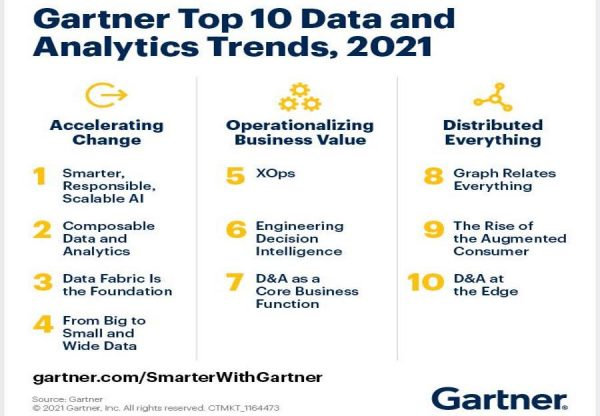
\includegraphics[scale=0.6]{img/fig13}
	\caption{Exemple de Word Count.}
\end{figure}
    \newpage
    \section*{Conclusion : }




    %\chapter{L'Internet des Objets (IoT) :}
\section*{Introduction}
Depuis la fin des années 1980, Internet a évolué de manière spectaculaire. La dernière étape est l’utilisation de ce réseau mondial pour la communication avec des objets ou entre objets, évolution nommée Internet des Objets (IoT pour Internet of Things).

L’évolution de l’IoT est rapide et n’a pas de limites, elle constitue la prochaine étape de la révolution numérique. En effet, depuis 2014, le nombre d’objets connectés est supérieur au nombre d’humains connectés et il est prévu que 50 milliards d’objets seront connectés en 2020.

\begin{figure}[h]
	\centering
    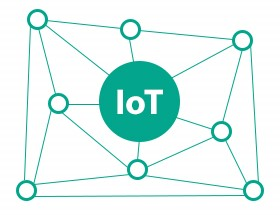
\includegraphics[scale=0.8]{img/part1/2.1}
    \caption{Internet of Things}
\end{figure}

\newpage
\section{Définition :}

\textbf{Définition 1 :} L’IoT (Internet of Things, pour Internet des Objets) est un système d’interconnexion entre des dispositifs informatiques, des machines, des objets, des animaux et même des personnes, munies d’identifiants uniques (UID) avec la capacité de transférer des données sur un réseau. Et ce, sans interaction d’humain à humain ou d’humain à ordinateur. 

Globalement, il s’agit de tout « objet » naturel ou artificiel auquel on peut attribuer une adresse IP et qui peut transférer des données sur un réseau. De plus en plus d’entreprises, quelque soit le secteur, utilisent l’IoT pour fonctionner plus efficacement et mieux comprendre leurs clients, afin d’offrir de meilleurs services. Mais aussi pour améliorer la prise de décision et accroître la valeur de l’entreprise.

\textbf{Définition 2:} L’internet des objets peut aussi être défini selon l’UIT, comme étant une infrastructure mondiale pour la société de l’information, qui permet de disposer de services évolués en interconnectant des objets (physiques ou virtuels) grâce aux technologies de l’information et de la communication interopérables existantes ou en évolution.
\section{L’histoire de l’IoT :}
C’est lors d’une présentation faite à Procter \& Gamble, en 1999, que Kevin Ashton, co-fondateur de l’Auto-ID Center au MIT, a mentionné pour la première fois l’Internet des Objets. Il souhaitait attirer l’attention des directeurs de P\& G sur les puces RFID (identification par radiofréquence). Cependant, il a nommé sa présentation « Internet of Things » pour intégrer la nouvelle tendance de l’année : Internet. Toutefois, l’idée d’appareils connectés existe depuis les années 1970. Ainsi, le premier objet connecté était une machine à Coca, à l’Université de Carnegie Mellon, au début des années 1980.

Via le Web, les développeurs pouvaient vérifier l’état de la machine, et déterminer si une boisson froide était disponible pour eux. L’IoT a ensuite évolué avec des technologies sans fil (Wifi par exemple), des MEMS (systèmes microélectromécaniques), des microservices et d’Internet. Ainsi, la technologie opérationnelle (OT – Operational Technology) et la technologie de l’information (IT) se sont rapprochées. Ceci a permis d’analyser des données non structurées, générées par des machines, pour en tirer des axes d’amélioration.

L’Internet des Objets utilise comme base la connectivité M2M (Machine to Machine). C’est-à-dire que des machines se connectent entre elles, via un réseau, sans interaction humaine. L’IoT est donc un réseau de milliards de noeuds (capteurs ici), qui connectent des personnes, des systèmes et d’autres applications pour collecter et partager des données. Néanmoins, le concept d’écosystème de l’Internet of Things ne s’est concrétisé qu’au milieu des années 2010. Une avancée que l’on doit au gouvernement chinois, qui a déclaré qu’il ferait de l’IoT une priorité stratégique, notamment dans sa stratégie de reconnaissance faciale et de fichage du peuple chinois.

\newpage
\section{les composantes d'un réseau IoT :}

Un système IoT réunit de nombreux acteurs et composants technologiques. Il est composé d'objets connectés, de réseaux de communication et de plateformes de services IoT pour les utilisateurs finaux.

\begin{figure}[h]
	\centering
    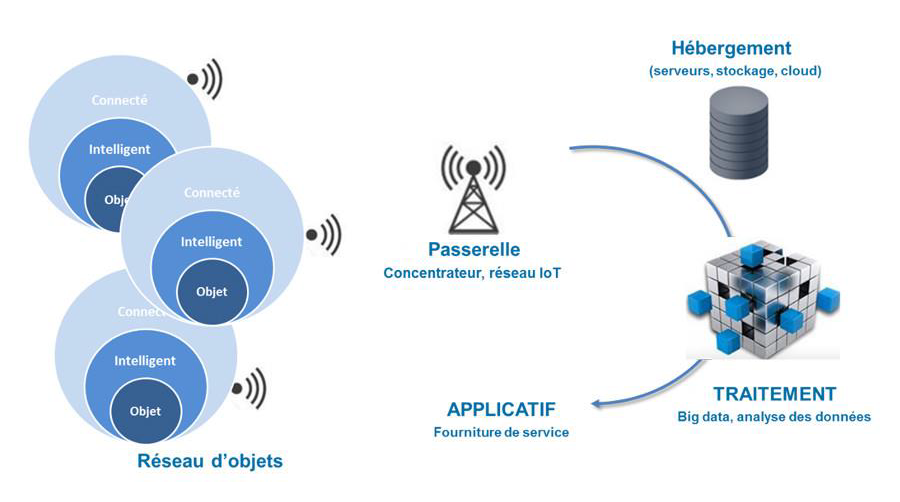
\includegraphics[scale=0.5]{img/part1/2.2}
    \caption{composantes d'un réseau IoT}
\end{figure}

\subsection{Les objets connecté:}
Les objets connectés sont des capteurs ou des objets dotés de capteurs capables de communiquer (envoyer et recevoir) des données à travers un réseau. Les données sont généralement envoyées à un ordinateur, une tablette, un smartphone ou tout autre appareil électronique et parfois via Internet pour que l’information soit accessible sur tous les appareils pouvant s’y connecter.

On distingue deux types d’objet :
\begin{itemize}[label=\textbullet]
\item \textbf{Les objets passifs :} ils utilisent généralement un tag (puce RFID, code barre 2D). Ils embarquent une faible capacité de stockage (de l’ordre du kilo-octet) leur permettant d’assurer un rôle . Ils peuvent parfois, dans le cas d’une puce RFID, embarquer un capteur (température, humidité) et être réinscriptibles.
\item \textbf{Les objets actifs :} ils peuvent être équipés de plusieurs de capteurs, d’une plus grande capacité de stockage, être doté d’une capacité de traitement ou encore être en mesure de communiquer sur un réseau.
\end{itemize}

\newpage 
\subsubsection{Exemples d’objets connectés}
Voici quelques objets connectés :
\begin{figure}[h]
	\centering
    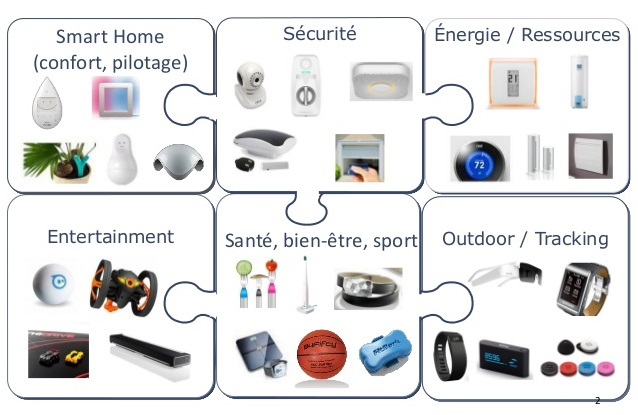
\includegraphics[scale=0.5]{img/part1/2.3}
    \caption{Exemples d’objets connectés}
\end{figure}
Comme on peut le voir on en retrouve de toute sorte : des appareils électroménagers comme les fours, les réfrigérateurs qui ont une capacité de se connecter à internet et de faciliter la vie des utilisateurs. Des camera connectée qui permettent aux utilisateurs via une application sur son Smartphone de vérifier en temps réel l'état de sa maison. Des Bracelets de santé connectés, des lunettes..etc

\subsubsection{Les composants d’un objet connecté :}
Les 4 composants essentiels, à la réalisation d’un objet connecté :
\begin{itemize}[label=\textbullet]
\item \textbf{Le capteur :} pour mesurer un paramètre extérieur tel qu’une température, un niveau d’humidité, un mouvement, un niveau de remplissage ou une pression atmosphérique… ou pour savoir si votre objet dysfonctionne, ou présente par exemple un défaut d’alimentation électrique. Tout débute par une prise d’information dans le monde physique. Bien sûr, l’objet peut intégrer plusieurs capteurs.

Il en existe de tout type: 
\begin{figure}[h]
	\centering
    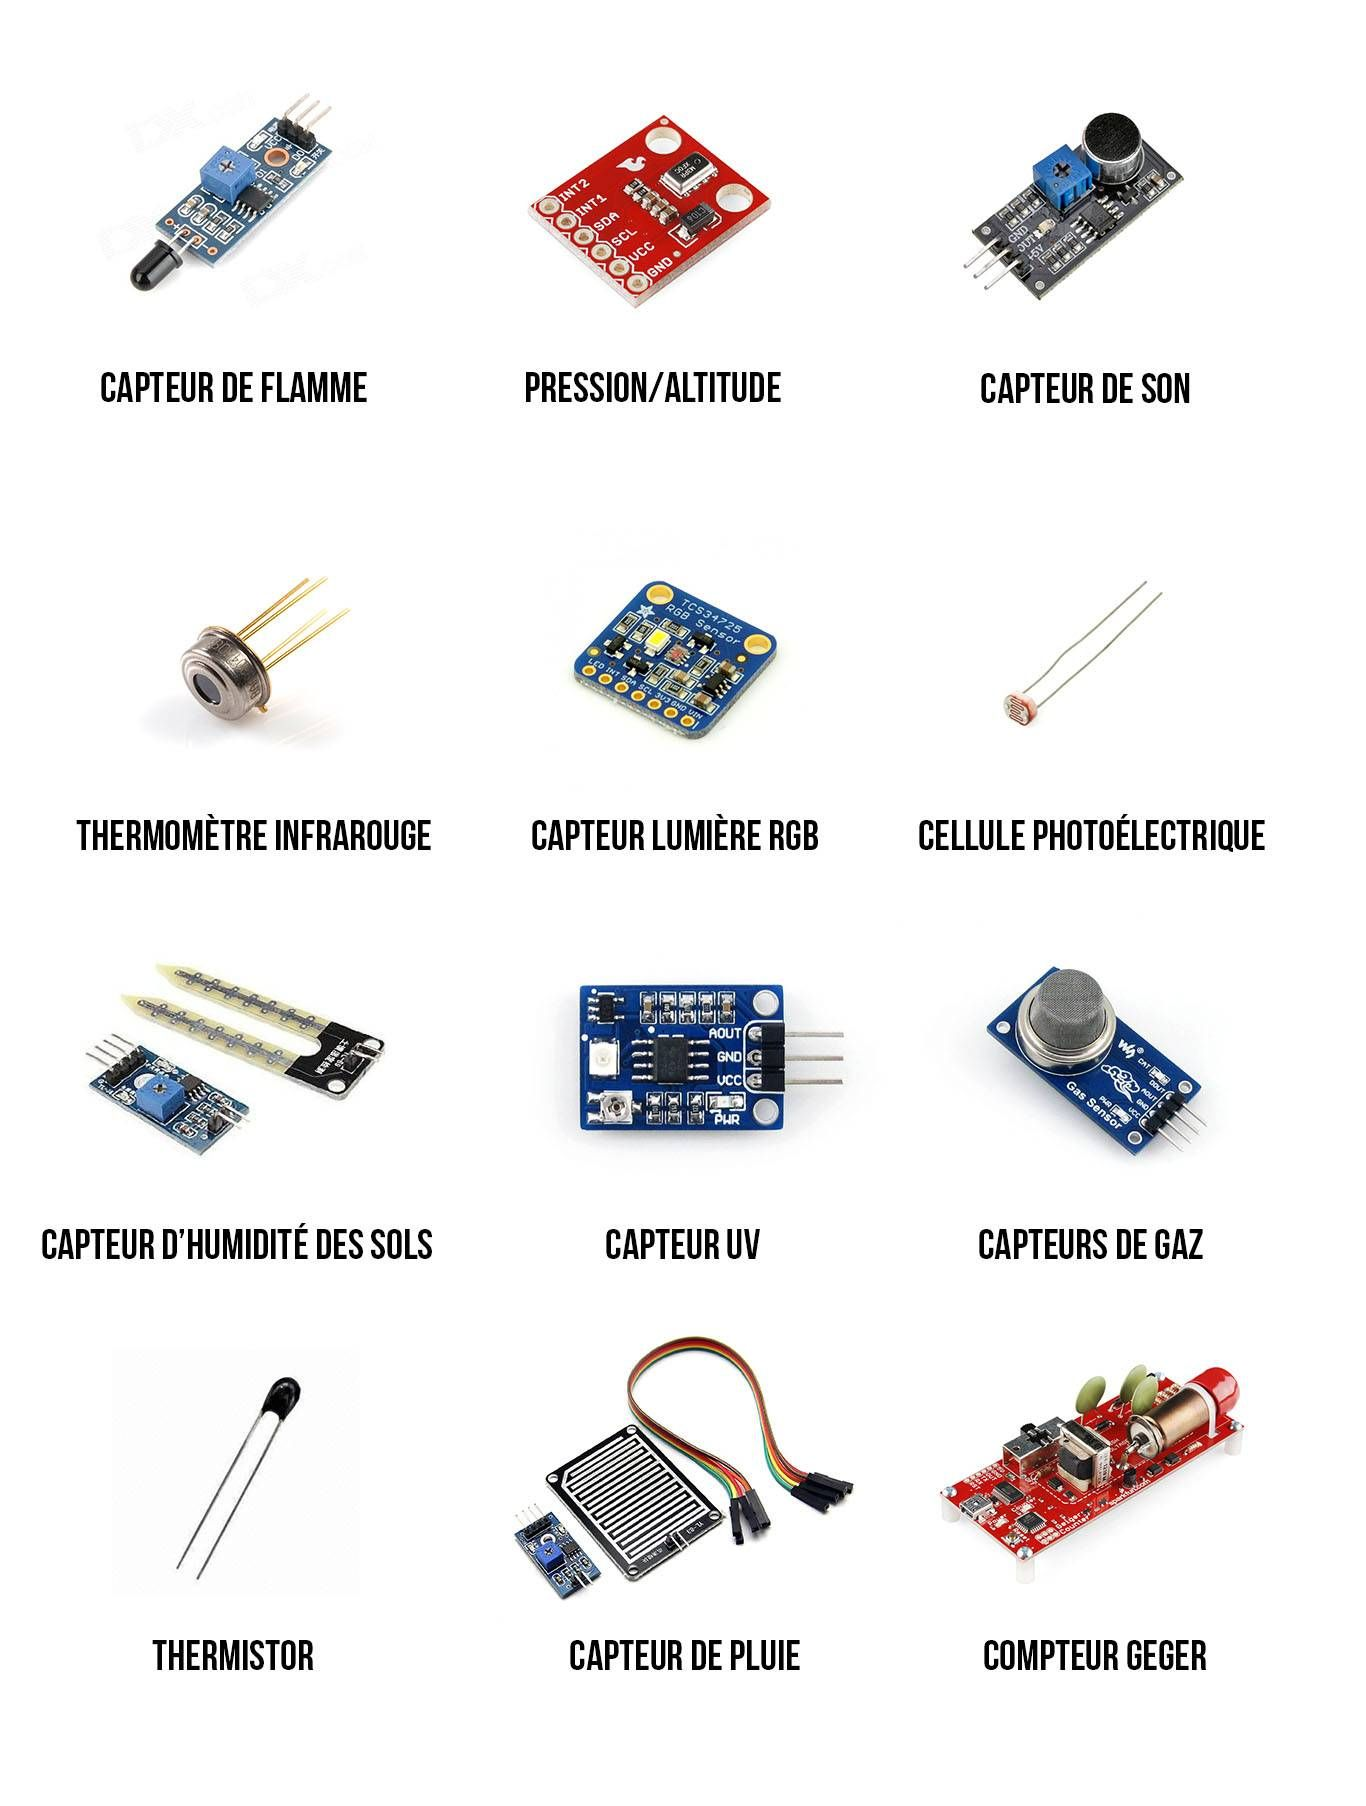
\includegraphics[scale=0.1]{img/part1/2.4}
    \caption{Exemples de capteurs}
\end{figure}

\item \textbf{Le logiciel embarqué :} Une fois l’information récupérée, il faut pouvoir stocker cette information et la traiter avant de la transmettre. C’est pour cela qu’on évoque parfois des objets « intelligents ». En effet, la plupart du temps, l’information est stockée localement, il s’agit d’attendre d’avoir plusieurs mesures successives ou de types différents et de les compiler pour pouvoir les transmettre.
\item \textbf{La puce de transmission :} lorsque l’information a été compilée, elle est prête à l’envoi. C’est à ce moment qu’intervient la puce de transmission. Celle-ci diffère en fonction du type de réseau, du volume d’informations à transmettre et de la vitesse de transfert.
\item \textbf{La batterie :} bien-sûr les objets connectés peuvent être alimentés par une prise électrique, mais la plupart du temps, ils sont autonomes. Dès lors, l’un des enjeux des ingénieurs est de réduire au maximum la dépense d’énergie des différents composants pour augmenter la durée de vie et/ou réduire la taille de l’objet. Le composant le plus énergivore est la puce de transmission. Ainsi, si votre objet transmet des informations à un rythme soutenu, vous risquez d’écourter sa durée de vie. C’est là qu’intervient l’intelligence embarquée permettant de ne transmettre que l’information pertinente et au moment où vous en avez besoin. De plus, les différents types de connectivité (Bluetooth, wifi, GSM, LPWA) ne sont pas équivalents en matière de consommation énergétique.
\end{itemize}

\subsection{Les réseaux de communication :}
Une fois capté, il est nécessaire de transporter la donnée vers internet. Ce transport peut se faire à l’aide de différents types de réseaux de communication. Ces réseaux seront utilisés en fonction du cas d’usage. Il faut donc choisir le réseau le plus adapté au cas d’usage requis car leur application va dépendre du débit souhaité. On peut alors les catégoriser en réseau haut débit ou bas débit.

Dans les réseaux hauts débits, on retrouve les réseaux habituels tels que les réseaux cellulaires (3G, 4G), Wifi et câblés (cuivre, fibre). En compléments, de nouveaux réseaux « bas débits » sont apparus depuis des années, donnant la possibilité à certains types d’objets d’être indépendant énergiquement et bénéficiant d’une longue portée de couverture radio. On les appelle les LPWAN – Low Power Wide Area Network. On retrouve notamment dans cette catégorie la technologie LoRa, déployée librement à l’échelle nationale par certains opérateurs , mais que l’on peut également déployer soi-même pour créer son propre réseau privé. Ce réseau permet une économie de la batterie des capteurs dans le but d’obtenir une autonomie de 2 à 10 ans et ainsi de réduire les coûts financiers de déploiement \& maintenance.

\begin{figure}[h]
	\centering
    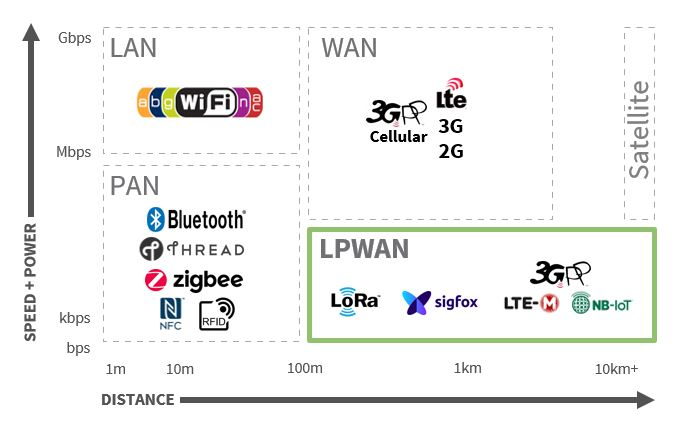
\includegraphics[scale=0.4]{img/part1/2.5}
    \caption{Réseaux de communication }
\end{figure}

\subsection{Les plateformes de service IoT:}
Après avoir créé et transmis la donnée, il faut l’analyser, la stocker et la restituer aux clients d’où la création d’une plateforme de services IoT. Certaines données sont directement exploitables tandis que d’autres nécessitent des « savoir-faire métier » pour transmettre des informations utiles et utilisables. Il existe donc deux types de plateformes sur le marché :
\begin{itemize}[label=\textbullet]
\item Les plateformes dites « verticales » vont traiter un cas d’usage spécifique très rapidement et proposent un ensemble de fonctionnalité (interface adaptée, notifications en temps réel, automatisation des rapports…). Par exemple, BH Technologies propose 2 solutions dans le but de gérer à distance l’éclairage public ainsi que la télérelève pour optimiser le ramassage des déchets au sein des villes.
\item Les plateformes dites « horizontales », génériques qui développent des applications sur mesure. Par exemple, la plateforme de NomoSense permet d’agréger des applications IoT de manière simple et ergonomique.
\end{itemize}

\begin{figure}[h]
	\centering
    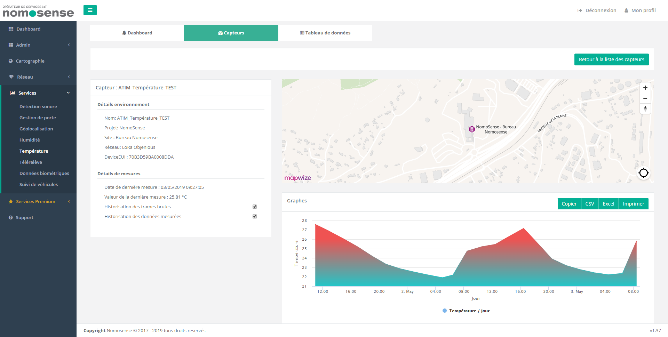
\includegraphics[scale=0.9]{img/part1/2.6}
    \caption{Les plateformes de service IoT}
\end{figure}
\newpage
\section{Architecture de l’Internet des objets}

%photo

Précisons le rôle des différents processus présentés sur ce schéma :
\begin{itemize}[label=\textbullet]
\item \textbf{Capter:} désigne l’action de transformer une grandeur physique analogique en un signal numérique.
\item \textbf{Concentrer:} permet d’interfacer un réseau spécialisé d’objet à un réseau IP standard (e.g. WiFi) ou des dispositifs grand public.
\item \textbf{Stocker:} qualifie le fait d’agréger des données brutes, produites en temps réel, méta taguées, arrivant de façon non prédictible.
\item \textbf{Présenter:} indique la capacité de restituer les informations de façon compréhensible par l’Homme, tout en lui offrant un moyen d’agir et/ou d’interagir.
\end{itemize}

Deux autres processus n’apparaissent pas sur le schéma, car ils sont à la fois transverves et omniprésents :
\begin{itemize}[label=\textbullet]
\item \textbf{Le traitement des données:} est un processus qui peut intervenir à tous les niveaux de la chaîne, depuis la capture de l’information jusqu’à sa restitution. Une stratégie pertinente, et commune quand on parle d’Internet des objets, consiste à stocker l’information dans sa forme intégrale. On collecte de manière exhaustive, « big data », sans préjuger des traitements qu’on fera subir aux données. Cette stratégie est possible aujourd’hui grâce à des architectures distribuées type NoSQL, capables d’emmagasiner de grandes quantités d’information tout en offrant la possibilité de réaliser des traitements complexes en leur sein (Map/Reduce par exemple).
\item \textbf{La transmission des données:} est un processus qui intervient à tous les niveaux de la chaîne.
\end{itemize}
\newpage
\section{La sécurité dans l'Internet des objets}

La sécurité de l’IoT est devenue l’objet d’un examen minutieux après un certain nombre d’incidents très médiatisés où un dispositif IoT commun a été utilisé pour infiltrer et attaquer un réseau plus important. La mise en œuvre de mesures de sécurité est essentielle pour garantir la sécurité des réseaux auxquels sont connectés des dispositifs IoT.

\subsection*{1. Les défis de l’IoT en matière de sécurité}
Un certain nombre de difficultés empêchent de sécuriser les dispositifs IoT et d’assurer la sécurité de bout en bout dans un environnement IoT. L’idée de mettre en réseau les appareils et autres objets étant relativement nouvelle, la sécurité n’a pas toujours été considérée comme une priorité absolue lors de la phase de conception d’un produit. En outre, comme l’IoT est un marché naissant, de nombreux concepteurs et fabricants de produits sont plus intéressés par une mise sur le marché rapide de leurs produits que par la prise des mesures nécessaires pour intégrer la sécurité dès le départ.

L’un des principaux problèmes cités en matière de sécurité de l’IoT est l’utilisation de mots de passe codés en dur ou par défaut, qui peut entraîner des failles de sécurité. Même si les mots de passe sont modifiés, ils ne sont souvent pas assez forts pour empêcher l’infiltration.

Un autre problème commun aux dispositifs IoT est qu’ils sont souvent à ressources limitées et ne contiennent pas les ressources de calcul nécessaires pour mettre en œuvre une sécurité forte. De ce fait, de nombreux dispositifs n’offrent pas ou ne peuvent pas offrir de fonctions de sécurité avancées. \textit{\textbf{Par exemple}, les capteurs qui surveillent l’humidité ou la température ne peuvent pas gérer un cryptage avancé ou d’autres mesures de sécurité.} De plus, comme de nombreux dispositifs de l’IoT sont « réglés et oubliés » – placés sur le terrain ou sur une machine et laissés en fin de vie – ils ne reçoivent pratiquement jamais de mises à jour ou de correctifs de sécurité. Du point de vue d’un fabricant, l’intégration de la sécurité dès le départ peut être coûteuse, ralentir le développement et empêcher le dispositif de fonctionner comme il le devrait.

La connexion d’actifs hérités qui ne sont pas intrinsèquement conçus pour la connectivité IoT constitue un autre défi en matière de sécurité. Le remplacement des infrastructures existantes par des technologies connectées est d’un coût prohibitif, c’est pourquoi de nombreux objets seront déjà équipés de capteurs intelligents. Cependant, les objets qui n’ont probablement pas été mis à jour ou qui n’ont jamais été sécurisés contre les menaces modernes sont toujours présents, la surface d’attaque potentielle est élargie.

En ce qui concerne les mises à jour, de nombreux systèmes ne prennent en charge qu’une période déterminée. En ce qui concerne les anciens et les nouveaux objets, la sécurité peut devenir caduque si une assistance supplémentaire n’est pas ajoutée. Et comme de nombreux dispositifs IoT restent sur le réseau pendant de nombreuses années, l’ajout de sécurité peut s’avérer difficile.

La sécurité de l’IoT souffre également d’un manque de normes acceptées par l’industrie. Bien qu’il existe de nombreux cadres de sécurité de l’IoT, il n’y a pas de cadre unique convenu. Les grandes entreprises et les organisations industrielles peuvent avoir leurs propres normes spécifiques, tandis que certains segments, tels que l’IoT industriel, ont des normes propriétaires incompatibles avec celles des leaders de l’industrie. La diversité de ces normes rend difficile non seulement la sécurisation des systèmes, mais aussi l’interopérabilité entre eux.

\subsection*{Violations de la sécurité de l’IoT et piratage de l’IoT}
Les experts en sécurité ont longtemps mis en garde contre le risque potentiel d’un grand nombre de dispositifs non sécurisés connectés à l’internet depuis que le concept d’IoT a vu le jour à la fin des années 1990. Un certain nombre d’attaques ont ensuite fait la une des journaux, allant des réfrigérateurs et des téléviseurs utilisés pour envoyer du spam à des pirates informatiques qui s’infiltrent dans les interphones pour bébés et parlent aux enfants. Il est important de noter que de nombreux pirates de l’IoT ne ciblent pas les appareils eux-mêmes, mais utilisent plutôt les appareils IoT comme point d’entrée dans le réseau général.

\textit{En 2010, \textbf{par exemple,} les chercheurs ont révélé que le virus Stuxnet avait été utilisé pour endommager physiquement des centrifugeuses iraniennes, les attaques ayant débuté en 2006 mais la principale ayant eu lieu en 2009. Souvent considéré comme l’un des premiers exemples d’attaque par l’IoT, Stuxnet vise les systèmes de contrôle de surveillance et d’acquisition de données (SCADA) dans les systèmes de contrôle industriel (SCI), en utilisant des logiciels malveillants pour infecter les instructions envoyées par les automates programmables (PLC).}

Les attaques contre les réseaux industriels n’ont fait que se poursuivre, avec des logiciels malveillants tels que CrashOverride/Industroyer, Triton et VPNFilter qui ciblent les systèmes OT et IoT industriels vulnérables.

En décembre 2013, un chercheur de la société de sécurité d’entreprise Proofpoint Inc. a découvert le premier botnet de l’IoT. Selon le chercheur, plus de 25 \% du botnet était constitué d’appareils autres que des ordinateurs, notamment des téléviseurs intelligents, des interphones pour bébés et des appareils ménagers.

En 2015, les chercheurs en sécurité Charlie Miller et Chris Valasek ont exécuté un piratage sans fil sur une Jeep, en changeant la station de radio du centre médiatique de la voiture, en mettant en marche ses essuie-glaces et son climatiseur, et en arrêtant l’accélérateur. Ils ont dit qu’ils pouvaient aussi couper le moteur, enclencher les freins et les désactiver complètement. Miller et Valasek ont pu infiltrer le réseau de la voiture grâce au système de connectivité embarqué de Chrysler, Uconnect.

Mirai, l’un des plus grands botnets de l’IoT à ce jour, a attaqué pour la première fois le site web du journaliste Brian Krebs et de l’hébergeur français OVH en septembre 2016. Les attaques ont atteint respectivement 630 gigabits par seconde (Gbps) et 1,1 térabit par seconde (Tbps). Le mois suivant, le réseau du fournisseur de services DNS (Domain Name System) Dyn a été pris pour cible, rendant un certain nombre de sites web, dont Amazon, Netflix, Twitter et le New York Times, indisponibles pendant des heures. Les attaques ont infiltré le réseau par le biais de dispositifs IoT grand public, notamment des caméras IP et des routeurs.

Un certain nombre de variantes de Mirai sont apparues depuis, notamment Hajime, Hide ‘N Seek, Masuta, PureMasuta, Wicked botnet et Okiru, entre autres.

Dans un avis de janvier 2017, la Food and Drug Administration (FDA) a averti que les systèmes intégrés dans les dispositifs cardiaques implantables de St. Jude Medical fonctionnant par radiofréquence, notamment les stimulateurs cardiaques, les défibrillateurs et les dispositifs de resynchronisation, pourraient être vulnérables aux intrusions et aux attaques de sécurité.

\subsection*{Outils et législation en matière de sécurité de l’IoT}
Il existe de nombreux cadres de sécurité pour l’IoT, mais il n’existe pas à ce jour de norme unique acceptée par l’industrie. Cependant, le simple fait d’adopter un cadre de sécurité pour l’IoT peut être utile ; il fournit des outils et des listes de contrôle pour aider les entreprises à créer et à déployer des dispositifs IoT. De tels cadres ont été publiés par la GSM Association, l’IoT Security Foundation, l’Industrial Internet Consortium et d’autres.

En septembre 2015, le Federal Bureau of Investigation a publié un message d’intérêt public, le numéro d’alerte du FBI I-091015-PSA, qui mettait en garde contre les vulnérabilités potentielles des dispositifs IoT et proposait des recommandations en matière de protection et de défense des consommateurs.

En août 2017, le Congrès a présenté la loi sur l’amélioration de la cybersécurité (IoT Cybersecurity Improvement Act), qui obligerait tout dispositif IoT vendu au gouvernement américain à ne pas utiliser de mots de passe par défaut, à ne pas présenter de vulnérabilités connues et à offrir un mécanisme pour corriger les dispositifs. Bien qu’elle vise les fabricants qui créent des dispositifs vendus au gouvernement, elle fixe une base de référence pour les mesures de sécurité que tous les fabricants devraient adopter.

Toujours en août 2017, la loi sur le développement de l’innovation et la croissance de l’Internet des objets (DIGIT) a été adoptée par le Sénat, mais attend toujours l’approbation de la Chambre. Ce projet de loi exigerait que le ministère du commerce convoque un groupe de travail et rédige un rapport sur l’IoT, notamment sur la sécurité et la protection de la vie privée.

Bien qu’il ne soit pas spécifique à l’IoT, le règlement général sur la protection des données (RPD), publié en mai 2018, unifie les lois sur la protection des données dans toute l’Union européenne. Ces protections s’étendent aux dispositifs IoT et à leurs réseaux, et les fabricants de dispositifs IoT doivent en tenir compte.

En juin 2018, le Congrès a présenté la loi sur l’état de l’application moderne, la recherche et les tendances de l’IoT, ou SMART IoT Act, pour proposer au ministère du Commerce de mener une étude sur l’industrie de l’IoT et de fournir des recommandations pour la croissance sécurisée des dispositifs IoT.

En septembre 2018, la législature de l’État de Californie a approuvé la loi SB-327 Information privacy : connected devices, qui a introduit des exigences de sécurité pour les dispositifs IoT vendus dans le pays.

Quelles sont les industries les plus vulnérables aux menaces à la sécurité de l’IoT ?
Les piratages de sécurité de l’IoT peuvent se produire dans n’importe quel secteur, de la maison intelligente à la voiture connectée en passant par une usine de fabrication. La gravité de l’impact dépend largement du système individuel, des données collectées et/ou des informations qu’il contient.

Une attaque désactivant les freins d’une voiture connectée, par exemple, ou sur un appareil de santé connecté, comme une pompe à insuline piratée pour administrer trop de médicaments à un patient, peut mettre la vie en danger. De même, une attaque sur un système de réfrigération abritant des médicaments qui est surveillé par un système IoT peut ruiner la viabilité d’un médicament si les températures fluctuent. De même, une attaque contre une infrastructure essentielle — un puits de pétrole, un réseau d’énergie ou un approvisionnement en eau — peut être désastreuse.

D’autres attaques, cependant, ne peuvent être sous-estimées. Par exemple, une attaque contre les serrures de portes intelligentes pourrait permettre à un cambrioleur d’entrer dans une maison intelligente. Ou encore, dans d’autres scénarios tels que le piratage de Target 2013 ou d’autres atteintes à la sécurité, un attaquant pourrait faire passer un logiciel malveillant par un système connecté – un système de chauffage, de ventilation et de climatisation dans le cas de Target – afin d’effacer des informations personnelles identifiables, causant ainsi des ravages pour les personnes concernées.

\subsection*{Comment protéger les systèmes et dispositifs IoT}

Les méthodes de sécurité de l’IoT varient en fonction de votre application spécifique de l’IoT et de votre place dans l’écosystème de l’IoT. Par exemple, les fabricants de l’IoT – des fabricants de produits aux entreprises de semi-conducteurs – doivent se concentrer sur l’intégration de la sécurité dès le départ, en rendant le matériel inviolable, en construisant du matériel sécurisé, en assurant des mises à jour sécurisées, en fournissant des mises à jour/rapports de micrologiciels et en effectuant des tests dynamiques. Les développeurs de solutions doivent se concentrer sur le développement de logiciels sécurisés et l’intégration sécurisée. Pour ceux qui déploient des systèmes IoT, la sécurité du matériel et l’authentification sont des mesures essentielles. De même, pour les opérateurs, il est essentiel de maintenir les systèmes à jour, d’atténuer les logiciels malveillants, de procéder à des audits, de protéger l’infrastructure et de sauvegarder les références.
\newpage
\section{Internet of Things : des applications pour tous ?}
Il existe de nombreuses applications de l’internet des objets. Cela va de l’IoT pour les industries de la grande consommation et de l’IoT entreprise à l’IoT manufacturier ainsi qu’à l’IoT industriel (IIoT). Ces applications couvrent de nombreux secteurs verticaux, notamment l’automobile, les télécommunications et l’énergie.

\subsubsection{1. Particuliers, bâtiments intelligents et sécurité publique}

Dans le segment des consommateurs, on peut citer les maisons intelligentes avec la domotique. Elles sont équipées de thermostats, d’appareils électroménagers, de chauffage, d’éclairage ou encore d’appareils électroniques intelligents. Ils peuvent tous être connectés et commandés à distance, via des ordinateurs, smartphones et autres appareils mobiles. Les bâtiments intelligents peuvent même réduire les coûts énergétiques grâce à des capteurs qui détectent le nombre d’occupants d’une pièce.

Du côté de la sécurité publique, des dispositifs portatifs permettent d’améliorer les délais d’intervention des permiers secours, en cas d’urgence, lors d’incendie par exemple ou lors d’une crise cardiaque d’une personne portant in pace maker. ou encore grâce à des itinéraires optimisés pour l’intervention des policiers ou du SAMU. Ou encore en suivant les signes vitaux des travailleurs de chantier ou des pompiers, sur des sites où leur vie est en danger. Dans le domaine de la santé, l’IoT permet de suivre les patients de plus près.

\subsubsection{2. Hôpitaux, smart cities et entreprises}

Les hôpitaux les utilisent aussi pour la gestion des stocks de produits pharmaceutiques et les instruments médicaux. En agriculture, l’Internet des Objets permet, par exemple, de surveiller la luminosité, la température, le taux d’humidité dans l’air et dans les sols des champs cultivés. Dans une smart city, ou ville intelligente, l’IoT se déploie à travers les réverbère intelligents et des compteurs intelligents. Ils permettent notamment de réduire la circulation et améliorer l’assainissement. Mais aussi réaliser des économies d’énergie et répondre aux préoccupations environnementales.

Pour les organisations, l’Internet des objets offre de multiples avantages, comme améliorer l’expérience client. Mais aussi, surveiller l’ensemble de leurs processus opérationnels, intégrer et adapter des modèles commerciaux et prendre de meilleures décisions. Ou encore améliorer la productivité des employés, économiser du temps et de l’argent, et générer plus de revenus. Globalement, l’IoT encourage les entreprises à repenser la manière dont elles abordent leurs activités, leurs industries et leurs marchés. Et il leur donne les outils nécessaires pour améliorer leurs stratégies commerciales.

\newpage
\section{Le rôle de l’Internet des objets dans le Big Data}
A mesure que le nombre d’objets connectés augmente, le volume de données générées par l’internet des objets explose. Ainsi, pour pouvoir les prendre en charge et les analyser en temps réel, il est nécessaire de s’en remettre aux outils analytiques Big Data.

Ces outils ont la capacité de traiter rapidement les larges volumes de données générées en continu par les appareils IoT, et d’en extraire des insights exploitables. Le machine learning permet notamment de repérer des modèles de données. Avec ces patterns, une entreprise peut notamment mettre en place la maintenance prédictive sur ses machines industrielles.

\textbf{Exemples de cas d’usage:}

\textit{Pour illustrer la corrélation entre IoT et Big Data, on peut prendre l’exemple des sociétés de transport. Ces dernières utilisent les données collectées par des capteurs et les outils d’analyse Big Data pour améliorer leur efficience, économiser de l’argent, et réduire leur impact sur l’environnement.}

\textit{Ou les véhicules de livraison embarquent des capteurs qui permettent de surveiller l’état du moteur, le nombre d’arrêts, la vitesse de déplacement, le nombre de kilomètres parcourus ou encore la quantité de carburant consommée.}

\newpage
\section{Le future de l'iot ? (Internet of Everything)}
L’Internet of Everything(IOE) (L’Internet du Tout) concerne et regroupe les connexions entre des personnes, des objets, des données et des processus pour former un système commun interdépendant dont le but est d’améliorer les expériences et de prendre des décisions plus éclairées.

Bien que le concept apparaisse comme un développement naturel du IoT, il englobe le concept plus large de connectivité : la philosophie de l’IoE décrit le monde dans lequel des milliards de capteurs sont implantés dans des milliards d’appareils, de machines et d’objets ordinaires, tous connectés sur des réseaux publics ou privés à l’aide de protocoles standard et propriétaires, ce qui leur confère de nombreuses opportunités de mise en réseau, les rendant ainsi plus intelligents.

Pour les entreprises, autant que pour les gouvernements et les particuliers, l’objectif principal de la technologie IoE est de convertir les informations collectées en actions, de faciliter la prise de décision basée sur des données.

\subsection{Caractéristiques de l'IOE :}
\begin{itemize}[label=\textbullet]
\item \textbf{Décentralisation :} Les données sont traitées non pas dans un seul centre, mais dans de nombreux noeuds distribués
\item \textbf{Entrée et sortie de données :} des données externes peuvent être injectées dans des périphériques et redistribuées au réseau.
\item \textbf{Relation avec toutes les technologies de transformation numérique :} Cloud computing, IA, Machine Leaning, IoT, Big Data, etc.
\end{itemize}

\subsection{Éléments constitutifs de l’IoE:}
\begin{enumerate}
\item \textbf{Personnes :} Considérées comme des noeuds finaux connectés sur Internet pour partager des informations et des activités, les personnes communiquent leurs points de vue personnels via des sites Web, des applications ou des appareils connectés qu’ils utilisent.

Ces données sont ensuite utilisées par des algorithmes d’intelligence artificielle et d’autres technologies intelligentes analysent ces données pour «comprendre» les problèmes humains et fournir un contenu pertinent en fonction de leurs besoins personnels ou professionnels.

\item \textbf{Les objets:} Ici, on parle de tous les objets connectés (capteurs physiques, dispositifs, actionneurs et autres éléments générant des données ou recevant des informations d’autres sources), donc le concept IoT pur.
\item \textbf{Les données:} Les données brutes générées par les périphériques et ensuite analysées puis traitées en informations, utiles pour permettre des décisions intelligentes et des mécanismes de contrôle; elles permettent d’autonomiser des solutions intelligentes, telle que l’évaluation des besoins en refroidissement d’une pièce, sur base de journaux de température précédents.
\item \textbf{Les processus:} Différents processus basés sur l’intelligence artificielle, l’apprentissage automatique, les réseaux sociaux ou d’autres technologies garantissent que les bonnes informations sont envoyées à la bonne personne au bon moment.

Le but des processus est de garantir la meilleure utilisation possible du Big Data. On peut citer ici par exemple, l’utilisation d’appareils de fitness intelligents et de réseaux sociaux pour annoncer des offres de soins de santé pertinentes à des clients potentiels.
\end{enumerate}

\subsection{La difference entre l’IOT et l’IOE :}
Les deux concepts d’IoT et d’IoE ne sont pas antagonistes. Bien au contraire, ils se complètent. L’Internet of Everything doit plutôt être considéré comme l’extension naturelle, comme la suite logique de l’Internet des objets. Rappelons qu’Internet est apparu par vagues successives. La première vague a consisté à connecter les ordinateurs (des militaires et scientifiques) entre eux avec le protocole IP. Puis la seconde vague a permis de connecter le grand public grâce à l’apparition du web, des réseaux mobiles, des réseaux sociaux, et à la démocratisation des PC personnels et des smartphones. La troisième vague est celle de l’IoT, qui vise à connecter tous les objets pouvant contenir un capteur. Au-delà des hommes et des ordinateurs, l’Internet des objets offre la possibilité inédite de connecter le monde physique dans son ensemble. Lorsque "tout" sera connecté, alors l’Internet of Everything sera devenu une réalité
\section*{Conclusion}
L’IoT est très certainement l’une des évolutions technologiques des plus remarquables étant donné son impact sur l’ensemble de notre société. L’utilisation d’objets connectés ne cesse d’évoluer et de s’accroitre dans divers secteurs et promet des découvertes des plus étonnantes mais comportent malgré tout certains risques. D’une part, des problèmes éthiques liés à la protection des données personnelles mais également de notre faculté à gérer nous-mêmes notre vie. Néanmoins, nous vivons dans un monde hyper connecté, et malgré certains inconvénients, l’internet des objets a encore de grands jours devant lui pour parer à ces éventualités.

    %\chapter{Le cloud computing :}
\section*{Introduction}
Depuis la fin des années 1980, Internet a évolué de manière spectaculaire. La dernière étape est l’utilisation de ce réseau mondial pour la communication avec des objets ou entre objets, évolution nommée Internet des Objets (IoT pour Internet of Things).

L’évolution de l’IoT est rapide et n’a pas de limites, elle constitue la prochaine étape de la révolution numérique. En effet, depuis 2014, le nombre d’objets connectés est supérieur au nombre d’humains connectés et il est prévu que 50 milliards d’objets seront connectés en 2020.

\begin{figure}[h]
	\centering
    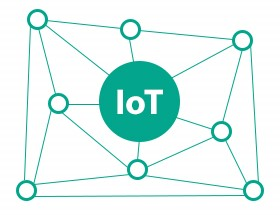
\includegraphics[scale=0.8]{img/3.1}
    \caption{Internet of Things}
\end{figure}


\section{Définitions}

\begin{description}
	\item[Définition 1:]« Le Cloud », littéralement le nuage, est un terme hérité du jargon technique. Aux débuts d'Internet, les diagrammes techniques représentaient souvent les serveurs et l'infrastructure réseau qui composent Internet sous la forme de nuages. Alors que de plus en plus de processus informatiques étaient déplacés vers cette partie 'serveurs et infrastructures' d'Internet, l'expression « passer dans le nuage » était une manière abrégée de désigner l'endroit où les processus informatiques se déroulaient. Aujourd'hui, « le cloud » est un terme largement accepté pour ce type d'accès.
	\item[Définition 2:] Le cloud computing est la fourniture de services informatiques notamment des serveurs, du stockage, des bases de données, la gestion réseau, des logiciels, des outils d'analyse, l'intelligence artificielle,  via Internet (le cloud) dans le but d'offrir une innovation plus rapide, des ressources flexibles et des économies d'échelle. 
	\item[Définition 3:] Un paradigme de calcul distribué émergeant dans lequel les données et les services
sont disponibles dans des data centers extensibles et peuvent être accédés de manière transparente depuis des appareils (ordinateurs, téléphones, grappes, ...) connectés par Internet.
\end{description}

De manière générale, on parle de Cloud Computing lorsqu’il est possible d’accéder à des données ou à des programmes depuis internet, ou tout du moins lorsque ces données sont synchronisées avec d’autres informations sur internet. Il suffit donc pour y accéder de bénéficier d’une connexion internet.
\newpage
\section{Les composants clés du cloud computing :}
Pour comprendre le fonctionnement du Cloud, il faut connaitre ses deux composants essentiels, à savoir la notion de Virtualisation et de Data center.

\subsection{Virtualisation :}
C'est l'ensemble des techniques matérielles et/ou logiciels qui permettent de faire fonctionner sur une seule machine, plusieurs systèmes d'exploitation (appelées machines virtuelles (VM), ou encore OS invité).

Même s'il existe plusieurs types de virtualisation, la forme la plus populaire de virtualisation dans le cloud est la virtualisation des serveurs qui consiste à dématérialiser le comportement et les données d'un serveur ou d'une machine, de façon à faire tourner plusieurs de ces instances dématérialisées sur un même serveur physique.

De cette façon, les diffiérentes instances créées se partagent les ressources du serveur physique. Cela permet une plus grande modularité dans la répartition des charges, une facilité dans l'administration des serveurs et une réduction des coûts.

\begin{figure}[h]
	\centering
	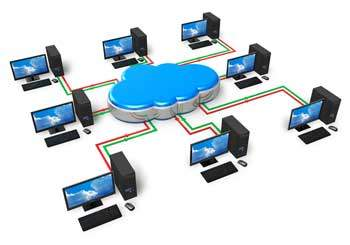
\includegraphics[scale=0.8]{img/part1/3.1}
	\caption{La Virtualisation}
\end{figure}

\subsection{Les Data Center :}
Un data center ou centre de données, c'est un site physique qui a une infrastructure composée d'un réseau d'ordinateurs et d'espaces de stockage, Il peut être interne ou externe à l'entreprise. Ces sites sont des salles remplies de baies de stockage, utilisées par de nombreuses entreprises et autres organisations gouvernementales

\begin{itemize}
\item  \textbf{Les composants du Data Center :} Un centre de données basique regroupe des serveurs, des sous-systèmes de stockage, des commutateurs de réseau, des routeurs, des firewalls, et bien entendu des câbles et des racks physiques permettant d'organiser et d'interconnecter tout cet équipement informatique.
\begin{figure}[h]
	\centering
	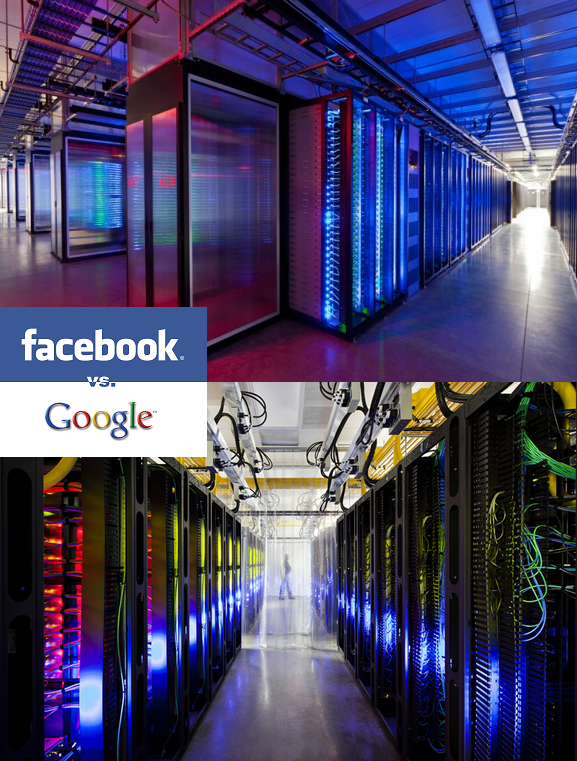
\includegraphics[scale=0.4]{img/part1/3.2}
	\caption{Exemple de data center (ceux de Facebook et Google)}
\end{figure}
\bigskip \bigskip \bigskip \bigskip
\item  \textbf{L'architecture du data center :} Théoriquement, n'importe quel espace suffisamment vaste peut servir de Data Center. Cependant, le design et l'implémentation d'un data center nécessite de prendre plusieurs précautions. Par-delà les problèmes basiques du coût et des taxes, les sites sont sélectionnés sur de nombreux critères, comme la localisation géographique, la stabilité météorologique, l'accès aux routes et aux aéroports, la disponibilité énergétique, les télécommunications ou encore l'environnement politique.

Pour fonctionner correctement, un Data Center doit aussi abriter l'infrastructure adéquate : un système distribution d'énergie, un commutateur électriques, des réserves d'énergie, des générateurs dédiés au backup, un système de ventilation et de refroidissement, et une puissante connexion internet. Une telle infrastructure nécessite un espace physique suffisamment vaste et sécurisé pour contenir tout cet équipement.
\end{itemize}
\begin{figure}[h]
	\centering
	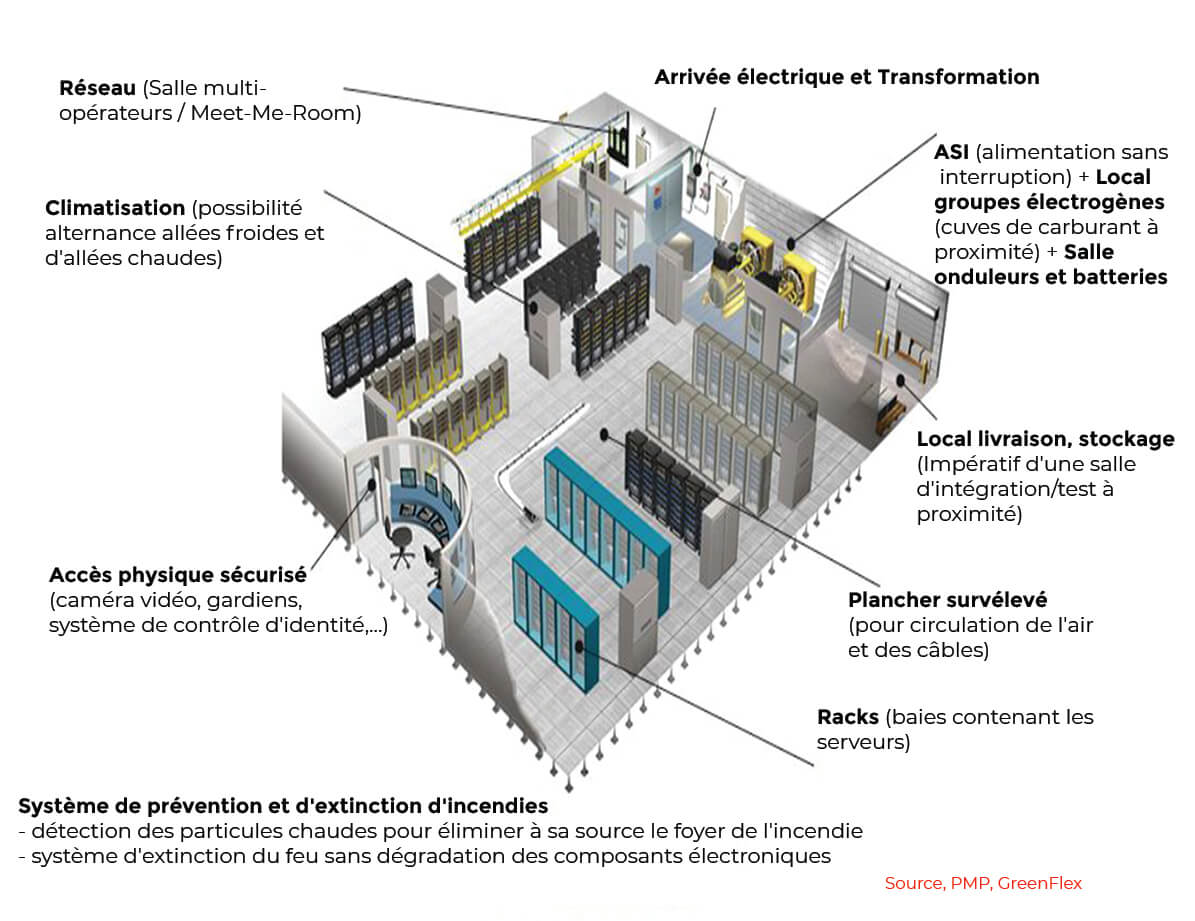
\includegraphics[scale=0.2]{img/part1/3.3}
	\caption{Architecture du data center}
\end{figure}





\newpage
\section{Utilisations du Cloud Computing}
Vous utilisez probablement en ce moment même le cloud computing sans le savoir. Si vous utilisez un service en ligne pour envoyer des courriers électroniques, modifier des documents, regarder des films ou regarder la télévision, jouer à des jeux ou stocker des images ou autres fichiers, il est probable que le cloud computing intervienne dans les coulisses. Les premiers services de cloud computing n’ont pas encore dix ans, mais un grand nombre d’organisations, par exemple des start-ups, des multinationales, des services administratifs ou des ONG, adopte cette technologie pour de nombreuses raisons.

Ici quelques exemples des possibilités d’utilisation des services cloud d’un fournisseur de cloud :

\begin{itemize}[label=\textbullet]
\item Créez des applications cloud natives Créez, déployez et mettez à l’échelle rapidement des applications (web, mobiles et API). Tirez parti des technologies et approches cloud natives, telles que les conteneurs, Kubernetes, l’architecture de microservices, la communication pilotée par des API et DevOps.
\item Tester et générer des applications Réduisez les coûts et délais de développement d’applications en utilisant des infrastructures cloud dont l’échelle peut être facilement adaptée.
\item Stocker, sauvegarder et récupérer des données Protégez vos données à moindre coût et à grande échelle en les transférant via Internet vers un système de stockage cloud hors site, accessible à partir de tout emplacement et appareil.
\item Analyser des données Unifiez vos données entre les équipes, les divisions et les emplacements dans le cloud. Utilisez ensuite des services cloud, par exemple de Machine Learning et d’intelligence artificielle, pour extraire des insights qui vous permettent de prendre des décisions éclairées.
\item Diffuser du contenu audio et vidéo Communiquez avec votre public en tout lieu, en tout temps et sur tout appareil via un système audio et vidéo haute définition mondialement distribué.
\item Incorporer de l’intelligence Utilisez des modèles intelligents pour interagir avec les clients et fournir des insights à partir des données capturées.
\item Diffuser des logiciels à la demande Également appelés logiciel en tant que service les logiciels à la demande vous permettent d’offrir à vos clients les versions et mises à jour les plus récentes des logiciels, à tout moment et en tout lieu.
\end{itemize}
\newpage
\section{Caractéristiques du Cloud}
Cette technologie offre plusieurs caractéristiques qui sont très avantageuse pour les utilisateurs professionnels et les utilisateurs finaux. Selon le NIST, le cloud computing doit posséder 5 caractéristiques essentielles qui sont: 

\begin{itemize}[label=\textbullet]
\item \textbf{Accès réseau universel :} L'ensemble des ressources doit être accessible et à disposition de l'utilisateur universellement et simplement à travers le réseau. 

\item \textbf{Libre service à la demande :} Permet à l'utilisateur d'utiliser et de libérer des ressources distantes en temps réel en fonction des ses besoins, sans nécessiter d'intervention humaine du côté fournisseur.

\item \textbf{Ressources partagées :} Les ressources matérielles du fournisseur sont partagées entre les différents utilisateurs.

\item \textbf{Élasticité :} Les ressources allouées aux utilisateurs peuvent être augmentées
ou diminuées selon l'usage.

\item \textbf{Service mesurable et facturable (pay-as-you-use) :} Les utilisateurs
paieront pour les ressources qu'ils ont utilisées et pour la durée de leur utilisation.
\end{itemize}

\section{inconvénients du Cloud}
Cette technologie offre plusieurs avantages et bénéfices pour les utilisateurs professionnels et les utilisateurs finaux. Les trois principaux avantages sont l’approvisionnement en libre-service, l’élasticité, et le paiement à l’utilisation.

Pour de nombreuses personnes, le stockage local utilisé pendant les dernières décennies demeure aujourd’hui supérieur au Cloud Computing. Ces personnes considèrent qu’un disque dur permet de garder les données et les programmes physiquement proches, autorisant un accès rapide et simplifié pour les utilisateurs de l’ordinateur ou du réseau local.

\subsection*{Faire confiance aux opérateurs}

C’est le principal reproche émis à l’égard du Cloud. Les télécoms, les entreprises de médias et les FAI contrôlent l’accès. Faire entièrement confiance au Cloud signifie également croire en un accès continu aux données sans aucun problème sur le long terme. Un tel confort est envisageable, mais son coût est élevé. De plus, ce prix continuera d’augmenter à mesure que les fournisseurs de Cloud trouvent un moyen de faire payer plus cher en mesurant par exemple l’utilisation du service. Le tarif augmente proportionnellement à la bande passante utilisée.

En dehors de ce problème de confiance, de nombreux autres arguments s’opposent au Cloud Computing. Le cofondateur d’Apple, Steve Wozniak, a ainsi critiqué le Cloud en 2012 en présageant de nombreux problèmes de grande envergure dans les cinq années à venir. On peut par exemple redouter des crashs. Durant l’été 2012, Amazon a rencontré ce type de problème. En tant que fournisseur d’entreprises comme Netflix ou Pinterest, l’entreprise américaine a ainsi provoqué la mise hors service des plateformes de ces clients. En 2014, Dropbox, Gmail, Basecamp, Adobe, Evernote, iCloud et Microsoft ont rencontré des problèmes similaires. En 2015, ce fut le tour de Apple, Verizon, Microsoft, AOL, Level 3, Google et Microsoft. Ces désagréments ne durent généralement que quelques heures, mais représentent une perte d’argent colossale pour les entreprises affectées.

\subsection*{La question de la propriété intellectuelle}
Par ailleurs, Wozniak a exprimé ses inquiétudes concernant la propriété intellectuelle. Il est en effet difficile de déterminer à qui appartiennent les données stockées sur internet. On peut prendre pour exemple les nombreuses controverses survenues au sujet des changements de conditions d’utilisation de sites dérivés du Cloud comme Facebook ou Instagram. Ces réseaux sociaux créent la polémique en s’octroyant des droits sur les photos stockées sur leurs plateformes. Il y a également une différence entre les données mises en ligne et les données créées directement au sein du Cloud. Un fournisseur pourrait aisément revendiquer la propriété de ces dernières. La propriété est donc un facteur à prendre en compte.

Aucune autorité centrale ne gouverne l’usage du Cloud pour le stockage et les services. L’Institute of Electrical and Electronics Engineers (IEEE) tente de devenir cet organe régulateur. En 2011, il a créé l’IEEE Cloud Computing Initiative, visant à établir des standards pour l’utilisation, particulièrement dans le domaine des entreprises. Pour l’heure, les règles sont encore floues et les problèmes se règlent au cas par cas.
\newpage
\section{Types de services Cloud}
La plupart des services de cloud computing peuvent être classés en trois grandes catégories : IaaS (infrastructure as a service), PaaS (platform as a service), SaaS (software as a service). On les appelle parfois « pile » de cloud computing, car elles s’empilent les unes sur les autres. Si vous savez en quoi elles consistent et en quoi elles sont différentes, vous pourrez plus facilement atteindre vos objectifs.
Ses derniers temps se rajoute a ses 3 services deux autres qu'on va présenter ci-dessous.

\begin{figure}[h]
	\centering
	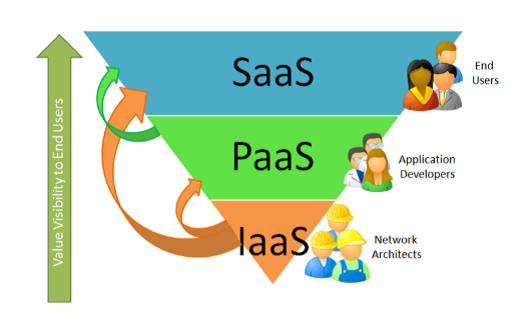
\includegraphics[scale=0.7]{img/part1/3.4}
	\caption{Services cloud}
\end{figure}

\begin{tabular}{|p{3cm}|p{6cm}|p{5cm}|} \hline
%1ere ligne
\textbf{Service}
& \textbf{Définition}
& \textbf{Exemple} \\ \hline

%2eme ligne
\begin{center}
Infrastructure as a service (IaaS)
\end{center} 
& 
La catégorie la plus basique des services de cloud computing. Avec l’IaaS, vous louez une infrastructure informatique (serveurs, machines virtuelles, stockage, réseaux, systèmes d’exploitation) auprès d’un fournisseur de services cloud, avec un paiement en fonction de l’utilisation.
& 
\begin{itemize}[label=\textbullet]
\item Amazon EC2 Elastic Compute Cloud.
\item S3 / Simple Storage Service d'Amazon.
\item Google drive, DropBox qui sont gratuits.
\end{itemize} 
\\ \hline

%3eme ligne
\begin{center}
Platform as a service (PaaS)  
\end{center}
& 
L’expression plateforme en tant que service (PaaS, Platform-as-a-Service) qualifie les services de cloud computing qui offrent un environnement à la demande pour développer, tester, fournir et gérer des applications logicielles. PaaS est conçu pour permettre aux développeurs de créer rapidement des applications web ou mobiles sans avoir à se préoccuper de la configuration ou de la gestion de l’infrastructure de serveurs, de stockage, de réseau et de bases de données nécessaire au développement. 
& 
\begin{itemize}[label=\textbullet]
\item App Engine de Google qui se limite à Java et Python.
\item Windows Azure de Microsoft permet de travailler avec les langages comme .NET, PHP, Python, Ruby et Java.
\end{itemize} 
\\ \hline
\end{tabular}

\begin{table}
\begin{tabular}{|p{3cm}|p{6cm}|p{5cm}|} \hline
%4ere ligne
\begin{center}
Software as a service (SaaS)  
\end{center}
& 
Le logiciel en tant que service (SaaS, Software-as-a-Service) est une méthode de diffusion d’applications logicielles via Internet, à la demande et en général sur abonnement. Avec le SaaS, les fournisseurs de services cloud hébergent et gèrent les applications logicielles et l’infrastructure sous-jacente, et gèrent la maintenance, par exemple la mise à niveau des logiciels et l’application des correctifs de sécurité. Les utilisateurs se connectent à l’application via Internet, en général par l’intermédiaire d’un navigateur web sur leur téléphone, leur tablette. 
& 
\begin{itemize}[label=\textbullet]
\item Google apps avec Google Docs, Calendar et Gmail qui sont gratuites.
\item Facebook, Linkdin qui sont gratuits.
\item Offices 365 de Microsoft propose des applications web (Word,Excel, PowerPoint, Publisher...).
\end{itemize} 
\\ \hline

%4ere ligne
\begin{center}
DBaaS (DataBase as a service ) 
\end{center}
& 
Un tel modèle fournit des mécanismes transparents pour créer, stocker, accéder et mettre à jour des bases de données. De plus, le fournisseur de services de base de données assume l'entière responsabilité de l'administration de la base de données, garantissant ainsi la sauvegarde, la réorganisation et les mises à jour de version. L'utilisation de ce service permet aux fournisseurs de répliquer et de personnaliser leurs données sur plusieurs serveurs, qui peuvent être physiquement séparé [16].
& 
\begin{itemize}[label=\textbullet]
\item Amazon Web Services.
\item RackSpace.
\item IBM, Microsoft, Oracle.
\end{itemize} 
\\ \hline

%4ere ligne
\begin{center}
Informatique serverless 
\end{center}
& 
Se chevauchant avec PaaS, l’informatique Serverless se concentre sur la création de fonctionnalités applicatives sans perte de temps en lien avec la gestion permanente des serveurs et de l’infrastructure requise à cette fin. Le fournisseur de cloud se charge de la configuration, de la planification de la capacité et de l’administration du serveur à votre place. Les architectures serverless sont hautement scalables et basées sur des événements. Elle n’utilisent des ressources que quand une fonction ou un déclencheur spécifiques s’activent.
& 
\begin{itemize}[label=\textbullet]
\item Google apps avec Google Docs, Calendar et Gmail qui sont gratuites.
\item Facebook, Linkdin qui sont gratuits.
\item Offices 365 de Microsoft propose des applications web (Word,Excel, PowerPoint, Publisher...).
\end{itemize} 
\\ \hline
\end{tabular}
\caption{Les services Cloud}
\end{table}
\newpage
\section{Types et modes de stockage dans le cloud computing :}
\subsection{Les types de stockage dans le cloud computing : }
Tous les clouds ne sont pas identiques et aucun type de cloud computing ne convient à tout le monde. Plusieurs modèles, types et services différents ont évolué pour nous aider à trouver la solution adaptée à vos besoins

\begin{itemize}[label=\textbullet]
\item \textbf{Cloud public :} est détenu et exploité par un fournisseur de cloud tiers, qui propose des ressources de calcul, telles que des serveurs et du stockage, via Internet. Microsoft Azure est un exemple de cloud public. Dans ce dernier, tout le matériel, tous les logiciels et toute l’infrastructure sont la propriété du fournisseur du cloud. Vous accédez à ces services et vous gérez votre compte par l’intermédiaire d’un navigateur web. 
\item \textbf{Cloud privé :} est l’ensemble des ressources de cloud computing utilisées de façon exclusive par une entreprise ou une organisation. Le cloud privé peut se trouver physiquement dans le centre de données local des entreprises, dans les quelles paient également des fournisseurs de services pour qu’ils hébergent leur cloud privé qui est un cloud dans lequel les services et l’infrastructure se trouvent sur un réseau privé. 
\item \textbf{Cloud hybride:} regroupe des clouds publics et privés, liés par une technologie leur permettant de partager des données et des applications. En permettant que les données et applications se déplacent entre des clouds privé et public, un cloud hybride offre à l’entreprise une plus grande flexibilité, davantage d’options de déploiement et une optimisation de l’infrastructure, de sécurité et de conformité existantes.
\item \textbf{Multicloud :} est un type de déploiement cloud qui implique l'utilisation de plusieurs clouds publics. Autrement dit, une organisation disposant d’un déploiement multi-cloud loue des serveurs et des services virtuels auprès de plusieurs fournisseurs externes. Les déploiements multi-cloud peuvent aussi être des clouds hybrides, et vice-versa.
\end{itemize}

\subsection{Les formats de stockage dans le cloud : }
Il existe trois formats de stockage de données dans le cloud :

\begin{itemize}[label=\textbullet]
\item \textbf{Stockage en mode bloc :} Le stockage en mode bloc permet de diviser un seul volume de stockage (par exemple, un nœud de stockage dans le cloud) en plusieurs instances individuelles appelées blocs. Il s'agit d'une solution de stockage rapide à faible latence, idéale pour les charges de travail hautes performances.
\item \textbf{Stockage en mode objet :} Le stockage en mode objet implique d'attribuer à chaque donnée des identifiants uniques, que l'on appelle les métadonnées. Compte tenu du fait que les objets ne sont ni compensés ni chiffrés, ils sont rapidement accessibles à très grande échelle. Il s'agit donc d'une solution idéale pour les applications cloud-native.
\item \textbf{Stockage en mode fichier :} Le stockage en mode fichier est le plus utilisé sur les systèmes NAS. Il permet d'organiser les données et de les présenter aux utilisateurs. Sa structure hiérarchique permet de parcourir les données du haut vers le bas en toute simplicité, mais augmente le temps de traitement.
\end{itemize}
\newpage
\section*{Conclusion:}
    %\chapter{Le NoSql :}
\section*{Introduction}
De nos jours, l’ubiquité de la connexion Internet est une réalité (les voitures que nous conduisons, les montres que nous portons, nos petits appareils médicaux domestiques, nos réfrigérateurs et congélateurs, nos Smartphones et ordinateurs portables). De plus, les données numériques produites par les êtres humains, dont les séquences vidéo, les photos et autres, atteignent des volumes importants de plusieurs EO par jour. 

Ces données actuellement stockées dans des bases qui leur ont été conçues spécifiquement sont gérés par des logiciels de gestion de bases de données volumineuses, jouant le rôle d’intermédiaires entre les bases de données d’un côté et les applicatifs et leurs utilisateurs de l’autre. On parle ici des bases de données non-relationnelles, dites NoSQL.

    
    \part{Conception}
    %\chapter{Smart Grid}
    \section*{Introduction}
Après plusieurs décennies de lente évolution, les réseaux électriques connaissent un développement
de grande envergure avec la multiplication des acteurs issus de la libéralisation des marchés
de l’énergie. Les préoccupations croissantes de sécurité d’approvisionnement et d’environnement,
les défis posés par le développement des énergies renouvelables et l’apparition de nouveaux usages
rendent les systèmes électriques de plus en plus complexes et donc vulnérables et plus chers en
exploitation. Lintroduction de plus d’intelligence grâce aux smart-grids est aujourd’hui le moyen
le plus efficace pour faire face à cette complexité croissante et résoudre les problèmes posés dans
les meilleures conditions de coût et de sûreté.

\begin{figure}[h]
	\centering
    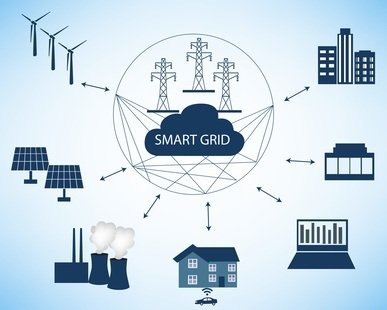
\includegraphics[scale=0.6]{img/part2/1.1}
    \caption{Le Smart Grid}
\end{figure}

    \newpage
    \section{Le réseau électrique intelligent Smart Grid}
    	\subsection{Définition:}
Le terme anglais « Smart Grid » (en français : « réseau intelligent ») désigne un système de distribution d’énergie électrique qui adapte automatiquement, en autonomie, la production à la demande.

Pour parvenir à cet équilibre en flux tendu, le Smart Grid fait appel à un réseau de capteurs, et à des dispositifs de transmission et d’analyse informatique des données en temps réel (ainsi qu’au Big Data), qui intègrent et infléchissent les modes de production et de consommation de manière à parvenir à un résultat optimal en matière d’efficacité énergétique et de sécurisation.

En d'autre terme les Smart Grid sont des réseaux d’électricité qui, grâce à des technologies informatiques, ajustent les flux d’électricité entre fournisseurs et consommateurs, et cela en collectant des informations sur l’état du réseau ils contribuent à une adéquation entre production, distribution et consommation.

Il est nécessaire de différencier smart grid et compteur communicant (ou « smart meter »), qui renseigne le consommateur sur sa demande en électricité. « Smart grids » est une appellation générale pour l’ensemble des technologies et des infrastructures « intelligentes » installées. Chez le particulier, le compteur communicant est une première étape dans la mise en place des smart grids.

\subsubsection*{Caractéristiques Du Smart Grid:}

Les réseaux intelligents peuvent être définis selon quatre caractéristiques en matière de :
\begin{itemize}[label=\textbullet]
\item \textbf{flexibilité :} ils permettent de gérer plus finement l’équilibre entre production et consommation ;
\item \textbf{fiabilité :} ils améliorent l’efficacité et la sécurité des réseaux ;
\item \textbf{accessibilité :} ils favorisent l’intégration des sources d’énergies renouvelables sur l’ensemble du réseau ;
\item \textbf{économie :} ils apportent, grâce à une meilleure gestion du système, des économies d’énergie et une diminution des coûts (à la production comme à la consommation).
\end{itemize}

\subsubsection{Objectifs}

Les objectifs des smart grids sont multiples et répondent à différentes exigences de leur part:
\\Réduire l'impact du système électrique sur l'environnement.
\begin{itemize}[label=\textbullet]
\item Eduquer les utilisateurs et à les rendre plus actifs quant à leur consommation d'électricité, tout en leur permettant de la contrôler efficacement
\item Développer la production d'électricité décentralisée.
\item Garantir un faible coût, efficace et sans coupure de courant.
\item Permet de gérer facilement le système électrique et de faire face à la complexité
croissante du système électrique
\end{itemize}
    	\newpage
    	\subsection{Passé et présent:}

Apparue dans les années 1980, la lecture automatique des compteurs (pour surveiller les charges électriques chez le consommateur) est une première étape dans l’émergence des smart grids.
Elle évolue dans les années 1990 vers le principe du compteur communicant, qui renseigne sur la variation de consommation électrique au cours de la journée. En 2000, le projet italien Telegestore est le premier exemple de smart grid. Par l’intermédiaire de ces compteurs, il relie au réseau un grand nombre de foyers (27 millions).

Le suivi et la synchronisation des réseaux sont été améliorés dans les années 1990 par la mise en place de capteurs analysant rapidement et à longue distance les anomalies électriques. Le premier système de mesure utilisant ce type de capteurs est opérationnel en 2000 aux États-Unis.
Aujourd’hui, les réseaux intelligents se développent progressivement. L’expression smart grids se généralise en 2005 avec la mise en place par la Commission Européenne de la plateforme technologique « Smartgrids ».

Les préoccupations environnementales et les attentes concernant la continuité de la fourniture d’électricité contribuent au déploiement de cette technologie. Les nombreux blackouts, notamment aux États-Unis ou en Italie, rappellent le besoin de moderniser des réseaux électriques très vieillissants.

Actuellement, malgré l’engouement des pouvoirs publics et des industriels, les implantations restent locales et parfois expérimentales. Le développement est progressif et l’adaptation des infrastructures prend du temps. En définitive, le développement des smart grids relève davantage d’une évolution dans l’optimisation des réseaux que d’une révolution technologique.
    	\newpage
    	\subsection{Fonctionnement:}
Au sens large, un réseau intelligent associe l’infrastructure électrique aux technologies numériques qui analysent et transmettent l’information reçue. Ces technologies sont utilisées à tous les niveaux du réseau : production, transport, distribution et consommation.

\begin{itemize}[label=\textbullet]
\item \textbf{Un contrôle des flux en temps réel :} des capteurs installés sur l’ensemble du réseau indiquent instantanément les flux électriques et les niveaux de consommation. Les opérateurs du réseau peuvent alors réorienter les flux énergétiques en fonction de la demande et envoyer des signaux de prix aux particuliers pour adapter leur consommation (volontairement ou automatiquement).

\item \textbf{L’interopérabilité des réseaux :} l’ensemble du réseau électrique comprend le réseau de transport et le réseau de distribution. Le premier relie les sites de production d’électricité aux zones de consommation : ce sont les grands axes qui quadrillent le territoire. Le réseau de distribution s’apparente aux axes secondaires. Il achemine l’électricité jusqu’aux consommateurs finaux. Par l’échange instantané d’informations, les smart grids favorise une interopérabilité entre les gestionnaires du réseau de transport et ceux du réseau de distribution.

\item \textbf{L’intégration des énergies renouvelables au réseau :} les réseaux intelligents reposent sur un système d’information qui permet de prévoir à court et à long terme le niveau de production et de consommation. Les énergies renouvelables qui fonctionnent souvent par intermittence et de façon peu prévisible peuvent ainsi être mieux gérées.

\item \textbf{Une gestion plus responsable des consommations individuelle :} les compteurs communicants (ou compteurs évolués, « Linky » pour l'électricité) sont les premières versions d’application du réseau intelligent. Installés chez les consommateurs, ils fournissent des informations sur les prix, les heures de pointe de consommation, la qualité et le niveau de consommation d’électricité du foyer. Les consommateurs peuvent alors réguler eux-mêmes leur consommation au cours de la journée. De leur côté, les opérateurs du réseau peuvent détecter plus vite les pannes.
\end{itemize}

\begin{figure}[h]
	\centering
    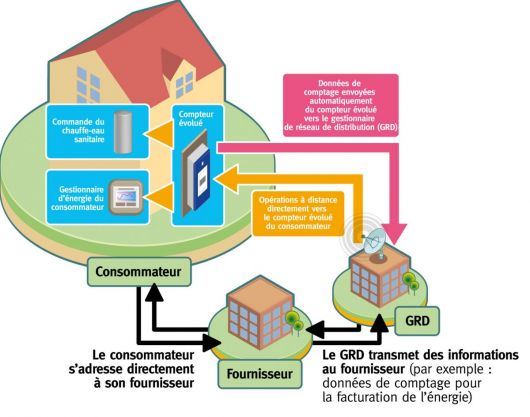
\includegraphics[scale=0.5]{img/part2/1.2}
    \caption{Fonctionnement du Smart Grid}
\end{figure}
    	\newpage
    	\subsection{Réseau classique VS Réseau électrique intelligent}
\noindent
\noindent
\begin{tabularx}{\linewidth}{|c|X|l|}
\hline
Caractéristiques des réseaux classiques & Caractéristiques des réseaux intelligents\\
\hline
Analogiques & Numériques\\ 
Unidirectionnel & Multidirectionnel\\ 
Production centralisé & Production décentralisé\\ 
Hiérarchique & Maillé\\ 
Peu instrumenté & Complètement instrumenté\\ 
Usagers & Clients\\ 
Un seul acteur économique & Choix du fournisseur\\ 
Peu de contrôle & Flexible\\ 
Gestion de l'équilibre par l'offre /production & Gestion de l'équilibre par demande/consommation\\ 
\hline
\end{tabularx}
    	
    	\subsection{Enjeux par rapport à l'énergie:}

À l’heure actuelle, les réseaux électriques doivent faire face à de nouveaux besoins en énergie, avec notamment le développement de la climatisation, des appareils électroniques ou du chauffage électrique. Cette hausse devrait être amplifiée par de nouveaux usages tels que la voiture électrique ou les pompes à chaleur. Les smart grids visent à apporter une réponse à ces contraintes.

\begin{enumerate}
\item \textbf{Des avantages économiques et environnementaux :}

Les smart grids améliorent la sécurité des réseaux électriques. En équilibrant l’offre et la demande, ils évitent le suréquipement des moyens de production et permettent une utilisation plus adaptée des moyens de stockage de l’électricité, disponibles de manière limitée.

Les réseaux intelligents augmentent aussi l’efficacité énergétique globale : ils réduisent les pics de consommation, ce qui atténue les risques de panne généralisée.
Enfin, ils limitent l’impact environnemental de la production d’électricité en réduisant les pertes et en intégrant mieux les énergies renouvelables.

\item \textbf{Les limites dans la mise en œuvre :}

Cependant, le coût des investissements reste élevé. En effet, les smarts grids doivent être implantés sur l’ensemble du réseau et impliquer tous les acteurs pour être efficaces.

L’autre obstacle est la diversité des acteurs, car ils doivent mettre au point des systèmes communicants variés avec des logiques convergentes. De plus, les données recueillies sont complexes à gérer et à stocker, compte tenu de l’importante quantité d’informations à traiter. 

Enfin, les informations sur les horaires ou les activités des consommateurs et des producteurs  sont confidentielles.  Des normes sur la protection des données doivent être appliquées. 
\end{enumerate}
    	\newpage
    	\subsection{Acteurs majeurs :}
Le développement des réseaux intelligents nécessite le concours  de nombreux acteurs :

\begin{itemize}[label=\textbullet]
\item \textbf{Les consommateurs:} en régulant eux-mêmes leur consommation d’électricité, participent à l’efficacité du système.

\item \textbf{Les producteurs d’électricité:} comme Sonalagaz en Algérie ou alors EDF en France alimentent les réseaux de transport  d’électricité et doivent être capables de répondre en temps réel à la demande. Le développement des smart grids permet également aux producteurs décentralisés de petites capacités (ex : les éoliennes ou les panneaux photovoltaïques appartenant à des particuliers) d’être raccordés.

\item \textbf{Les gestionnaires des réseaux de transport et de distribution ainsi que les constructeurs de matériel électrique} qui gèrent et installent les équipements de mesure assurant la sécurité et le fonctionnement des réseaux Ils sont les acteurs techniques majeurs du développement des smart grids.

\item \textbf{Les gestionnaires de processeurs et de systèmes informatiques:} comme InfoVista, Intel, Google ou Cisco System, développent les technologies d’information indispensables au fonctionnement des réseaux intelligents.

\item \textbf{Les pouvoirs publics:} soutiennent et encadrent le développement des réseaux intelligents notamment par la d1éfinition de normes de communication et la protection des systèmes contre les intrusions ou détournements.
\end{itemize}

\begin{figure}[h]
	\centering
    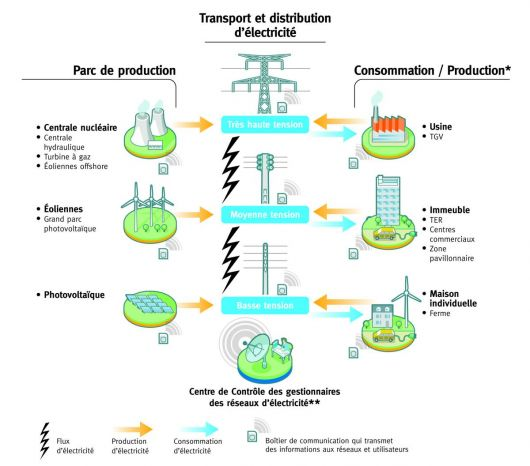
\includegraphics[scale=0.6]{img/part2/1.3}
    \caption{Intervention des acteurs dans le fonctionnement du Smart Grid.}
\end{figure}
    	\newpage
    	\subsection{Zone de présence ou d'application :}
À court et moyen termes, les réseaux intelligents seront essentiellement déployés dans les pays développés car la modernisation du réseau nécessite d’importants investissements 

Les États-Unis ont été précurseurs dans le développement des smart grids. De grands investissements sont en effet consentis afin de moderniser un réseau électrique défaillant et souvent obsolète.

En Europe, le niveau des avancées varie selon les pays. Les pays dont les réseaux sont fragiles et dont la production est largement émettrice de CO2 sont les plus volontaires (comme l’Italie et l’Espagne), tout comme ceux qui ont des préoccupations écologiques anciennes comme la Suède. La France dont le réseau est plutôt de bonne qualité et dont le parc de production est peu émetteur de CO2 affiche des objectifs plus lents.

Les investissements entrepris et les avancées réalisées concernent principalement l’installation de compteurs intelligents à ce jour. On estime à 80 \% le nombre de foyers qui pourraient théoriquement être équipés de compteurs intelligents d’ici 2020 en Europe. Il s’agit d’une condition indispensable mais non suffisante pour avoir des réseaux intelligents réellement efficaces. L’effort devra être conduit en parallèle sur les autres composants du réseau, notamment son système d’information.

Pour ce qui est de l'algérie Sonelgaz a développé la télérelève avec la généralisation des compteurs intelligents (smart meters) pour les clients en HTA.

\subsection{Futur des Smart Grid}
À long terme, le développement des smart grids devrait s’étendre à l’ensemble des réseaux interconnectés.

Toutefois, l’implantation des réseaux intelligents dépend de l’efficacité des dispositifs techniques et de l’implication des parties prenantes.

Parmi elles, les consommateurs auront un rôle clé. En effet, l’équilibre du système électrique sera davantage géré par l’utilisateur final. Une sensibilisation du public sur les enjeux du système sera alors nécessaire pour en comprendre l’utilité. Cela exigera aussi un accès aisé aux informations via des interfaces multiples et simples (smartphones, ordinateurs, etc.).

Au niveau politique, la Plateforme Technologique de l’Union européenne finance le développement des réseaux intelligents. Aux Etats-Unis, 4,5 milliards de dollars ont été investis dans la modernisation des réseaux prévue par l’American Recovery and Reinvestment Act de 2009.
    	\newpage
    	
    \section{Le compteur intelligent}
    	\subsection{Définition}
Un compteur intelligent est un compteur électronique qui mesure la quantité d'énergie consommée sur une période de temps définie. Il communique et transmet également des données de consommation, comme vos index, et peut recevoir des informations ou des ordres à votre demande. Il offre ainsi de nouveaux services sans rendez-vous et sans dérangement pour vous. 

Tous les compteurs intelligents affichent en permanence 4 index, peu importe que vous ayez une production d'énergie (par exemple, des panneaux photovoltaïques) et peu importe votre choix tarifaire (simple tarif, bi-horaire,...)  : 

\begin{itemize}[label=\textbullet]
\item la consommation aux heures pleines 
\item la consommation aux heures creuses 
\item l'injection d'énergie aux heures pleines 
\item l'injection d'énergie aux heures creuses
\end{itemize}

\begin{figure}[h]
	\centering
    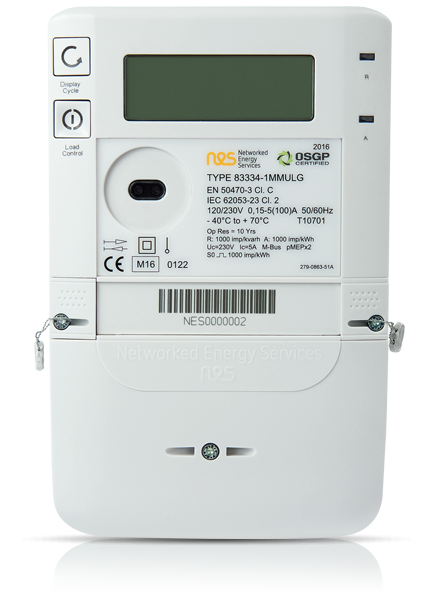
\includegraphics[scale=0.4]{img/part2/1.4}
    \caption{Exemple de compteur intelligent}
\end{figure}
    	\newpage
    	\subsection{Fonctionnement}
Contrairement aux compteurs électro-mécaniques qui doivent être relevés manuellement, les compteurs intelligents :

\begin{itemize}[label=\textbullet]
\item Enregistrent dans leur mémoire, selon un protocole défini, la puissance électrique prélevée et les quantités consommées à différents moments de la journée chaque jour de la semaine.
\item Transmettent de manière électronique ces données au gestionnaire de réseau  ou au client.
\item Peuvent être contrôlés et vérifiés à distance par le gestionnaire de réseau.
\item Envoient une alarme au gestionnaire de réseau en cas d’ouverture du capot et donc, de suspicion de fraude.
\end{itemize}

\begin{figure}[h]
	\centering
    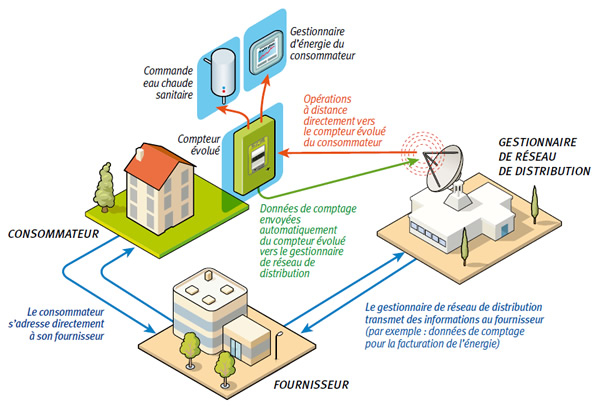
\includegraphics[scale=0.6]{img/part2/1.5}
    \caption{Fonctionnement du compteur intelligent}
\end{figure}
    	\newpage
    	\subsection{Les avantages et les inconvénient}

\subsubsection{Avantages du compteur intelligent}
Le compteur intelligent offre plusieurs avantages aux consommateurs :
\begin{itemize}[label=\textbullet]
\item Les démarches sont facilitées 
\item Fini le passage d'un technicien pour le relevage du compteur, la consommation étant communiquée en temps réel au distributeur ;
\item Une consommation raisonnée et davantage écoresponsable ;
\item Une facturation suivie et dimensionnée quotidiennement grâce aux facilités de suivi, et donc plus précise.
\end{itemize}

En bref, le compteur intelligent permet un relevé automatique et précis à distance. En effet, avec ce type de compteur, le fournisseur peut commander vos appareils à distance et suivre toutes vos consommations.

\subsubsection{Ses inconvénients : des craintes plus ou moins fondées ?}
De nombreuses voix se sont opposées aux compteurs intelligent. Cependant, les raisons invoquées ne sont pas toutes avérées. Cette méfiance n'en est pas moins à prendre en compte, et révèle la nécessité de mettre en place des études et des contrôles réguliers et indépendants.

\begin{itemize}[label=\textbullet]
\item Première crainte, les radiofréquences CPL (courant porteur en ligne) injectées par les compteurs dans les câbles et appareils électriques. Ce type de technologie est également utilisé en domotique, pour les réseaux internet, etc. Certaines associations affirment que le CPL est dangereux pour la santé, mais 60 Millions de Consommateurs met en garde : pour le moment, aucune étude n'est parvenue à prouver cette dangerosité.
\item Deuxième point de méfiance : des pannes et des incendies ont déjà été observés sur les appareils en service. De fait, durant la phase test, 8 incendies ont été imputés non pas au compteur lui-même mais à des erreurs de manipulation pendant la pose (sur 300 000 installations). Des précisions qui rassurent quant à la capacité des installateurs à limiter ce risque.
\item Enfin, la surveillance généralisée des faits et gestes de la population est rendue possible par la transmission en temps réel des données de consommation, ce qui peut poser problème à certains. Néanmoins, c'est grâce à cette collecte d'informations que la domotique peut simplifier votre quotidien : mieux elle vous connaît, mieux elle peut agir pour vous. De plus, les données relevées par les compteurs intelligents sont surveillées par la CNIL, et soumises à des règles strictes.
\end{itemize}
    	\newpage
    	
	\section{Le Smart Grid et big data}
    	




    \chapter{Etude et Conception}
    \section*{Introduction}
Nous abordons maintenant une question très importante dans le cadre de la mise en œuvre d’une grande base de données : comment modéliser cette dernière pour satisfaire les besoins de l’application? Et plus précisément:

\begin{itemize}[label=\textbullet]
\item quelle est la structure des données?
\item Quelles sont les contraintes qui portent sur le contenu de nos tables? 
\end{itemize}

Cette question est bien connue dans le contexte des bases de données relationnelles. Pour les bases NoSQL, il n’existe pas de méthodologie équivalente. Une bonne (ou mauvaise) raison est d’ailleurs qu’il n’existe pas de modèle normalisé, et que la modélisation doit s’adapter aux caractéristiques de chaque système.

Voyons comment on pourrait modéliser notre base de données avec Cassandra. Notre démarche consiste à:
\begin{itemize}[label=\textbullet]
\item Déterminer les « entités » (Clients, Compteur, Capteurs..etc ) pertinentes pour l’application.
\item Définir une méthode d'identification de chaque entité.
\item Préserver le lien entre les entités.
\end{itemize}


    \newpage
    \section{Réflexion sur la modélisation d'un Smart Grid}
Dans le contexte de l'amélioration de la situation de travail chez Sonelgaz, On a imaginé un système permettant de récolter les données des compteurs électrique plus facilement dans les différents scénarios suivant:

\subsection{Cas normal:}
Le premier scénario qui peut se produire sur notre système est assez simple, c'est le fait que le capteur d'index se charge d'envoyer des données toutes les minutes vers la base de données et de stocker ces dernières.

Dans ce scénario aucune erreur n'est captée, ce qui fait que le capteur d'erreurs n'envoie aucune donnée, par la suite les utilisateurs pourrons vérfié et suivre leur consommation sur l'application. Le schéma suivant illustre ce cas:

\begin{figure}[h]
	\centering
	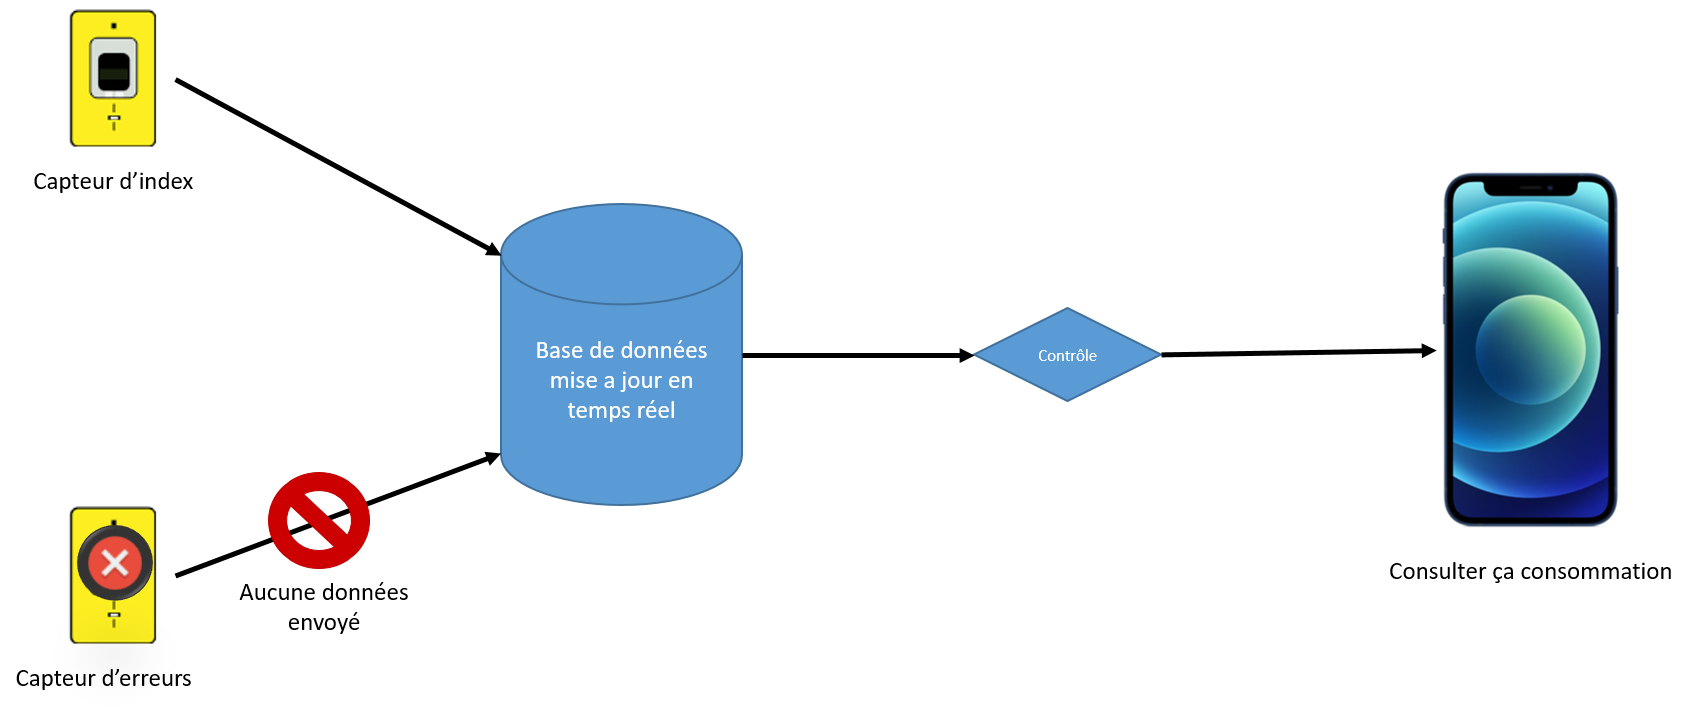
\includegraphics[scale=0.6]{img/part2/2.1.png}
	\caption{Scénario normal}
\end{figure}

\newpage

\subsection{Cas d'erreurs:}
Pour le deuxième scénario, se produit lorsqu'une erreur est détectée, le capteur d'index continue d'envoyer des données, en plus du capteur d'erreur qui intervient également en envoyant des données sur l'erreur qui s'est produite. notre système réagit différemment selon l'erreur captée:

\begin{itemize}
	\item \textbf{Surconsommation d'énergie:}

	\item \textbf{Ouverture du compteur:}

	\item \textbf{arrêt inattendu:}

	\item \textbf{Non payement:}

\end{itemize}

Le schéma suivant illustre ce cas avec les différentes erreurs:

\begin{figure}[h]
	\centering
	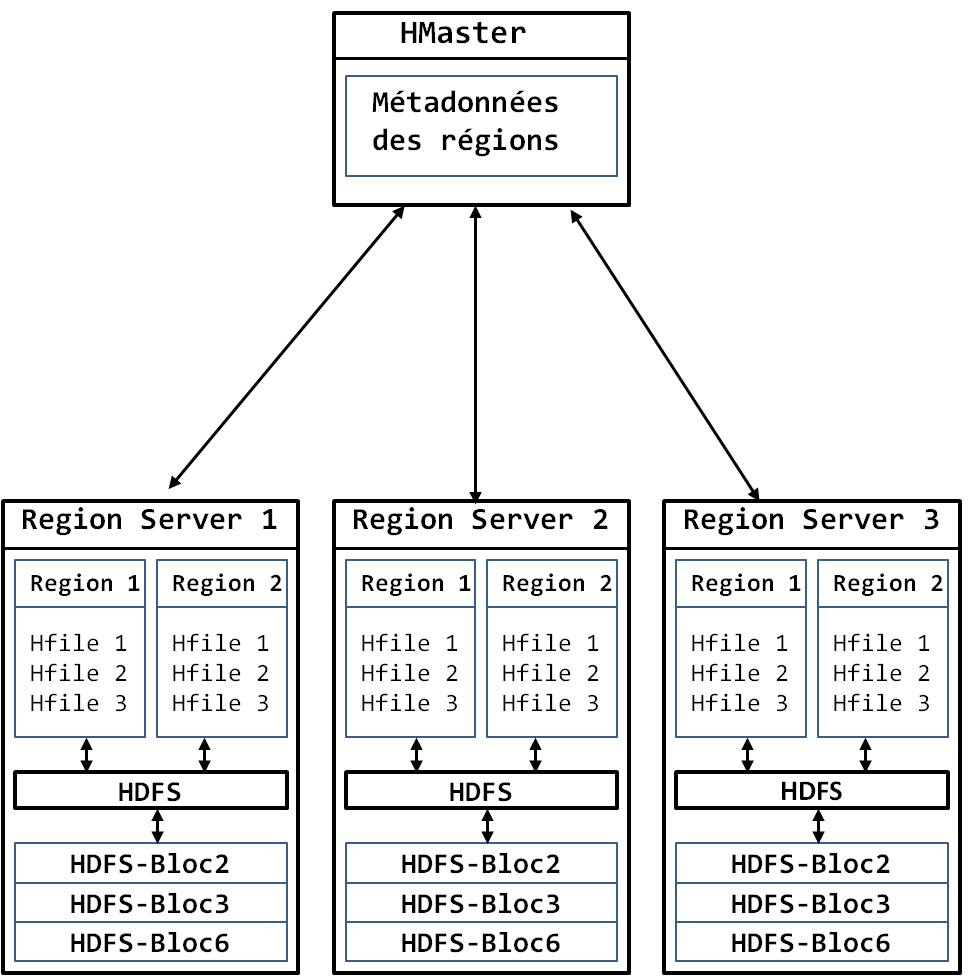
\includegraphics[scale=0.5]{img/part2/2.2.png}
	\caption{Scénario erreur}
\end{figure}

    \newpage
    \section{La Collecte des données relatives a ce système}

Après avoir délimiter notre projet selon nos besoins et étudier le contexte ainsi que la description des scénarios susceptibles de générer de la valeur. Nous venons ici collecter ces données relatives a ce pays.

Par collecte de données, on entend l'approche systématique qui consiste a réunir et a mesurer des informations en provenance des compteurs, afin d'obtenir une vue complété et précise de la consommation d'énergie. La collecte des données permet aux utilisateurs ou a l'entreprise Sonelgaz de répondre a des questions pertinentes, d'évaluer des résultats et de mieux anticiper les probabilités et les tendances a venir. 

Dans le cadre de notre travail on va classer ces données en deux catégories a savoir:

\textbf{Les données fixes :} Une donnée fixe est en général immuable c'est-a-dire son état ne peut être modifier au fil du temps.

\textbf{Les données évolutives :} On dit qu'une donnée est évolutive si dans un même
contexte, sa valeur change au fil du temps.

Selon notre contexte a étudier, Les données sur lesquelles nous informe ce système sont regroupées dans le tableau suivant :

\begin{figure}[h]
	\centering
	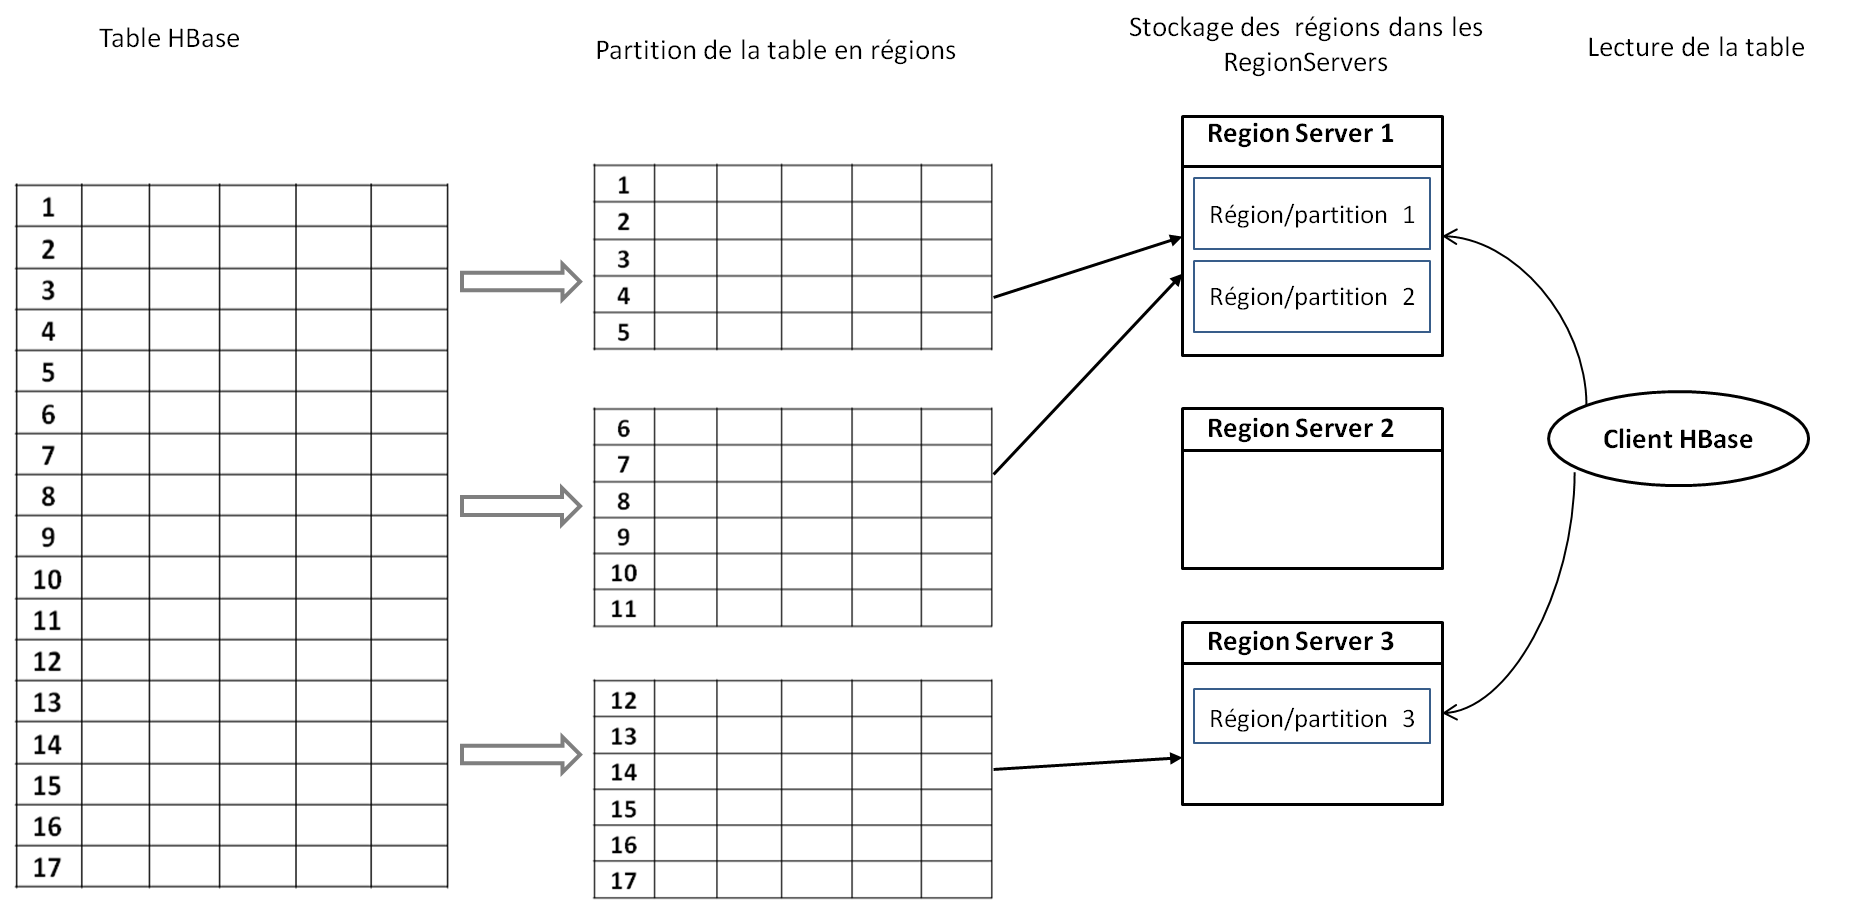
\includegraphics[scale=0.8]{img/part2/2.3.png}
	\caption{Exemple de donnees collectees}
\end{figure}

    \newpage
    \section{Structuration des données récoltées pour Cassandra:}

Le modèle utilisé pour structurer nos données pour Cassandra est le modèle orientée colonnes.

\begin{figure}[h]
	\centering
	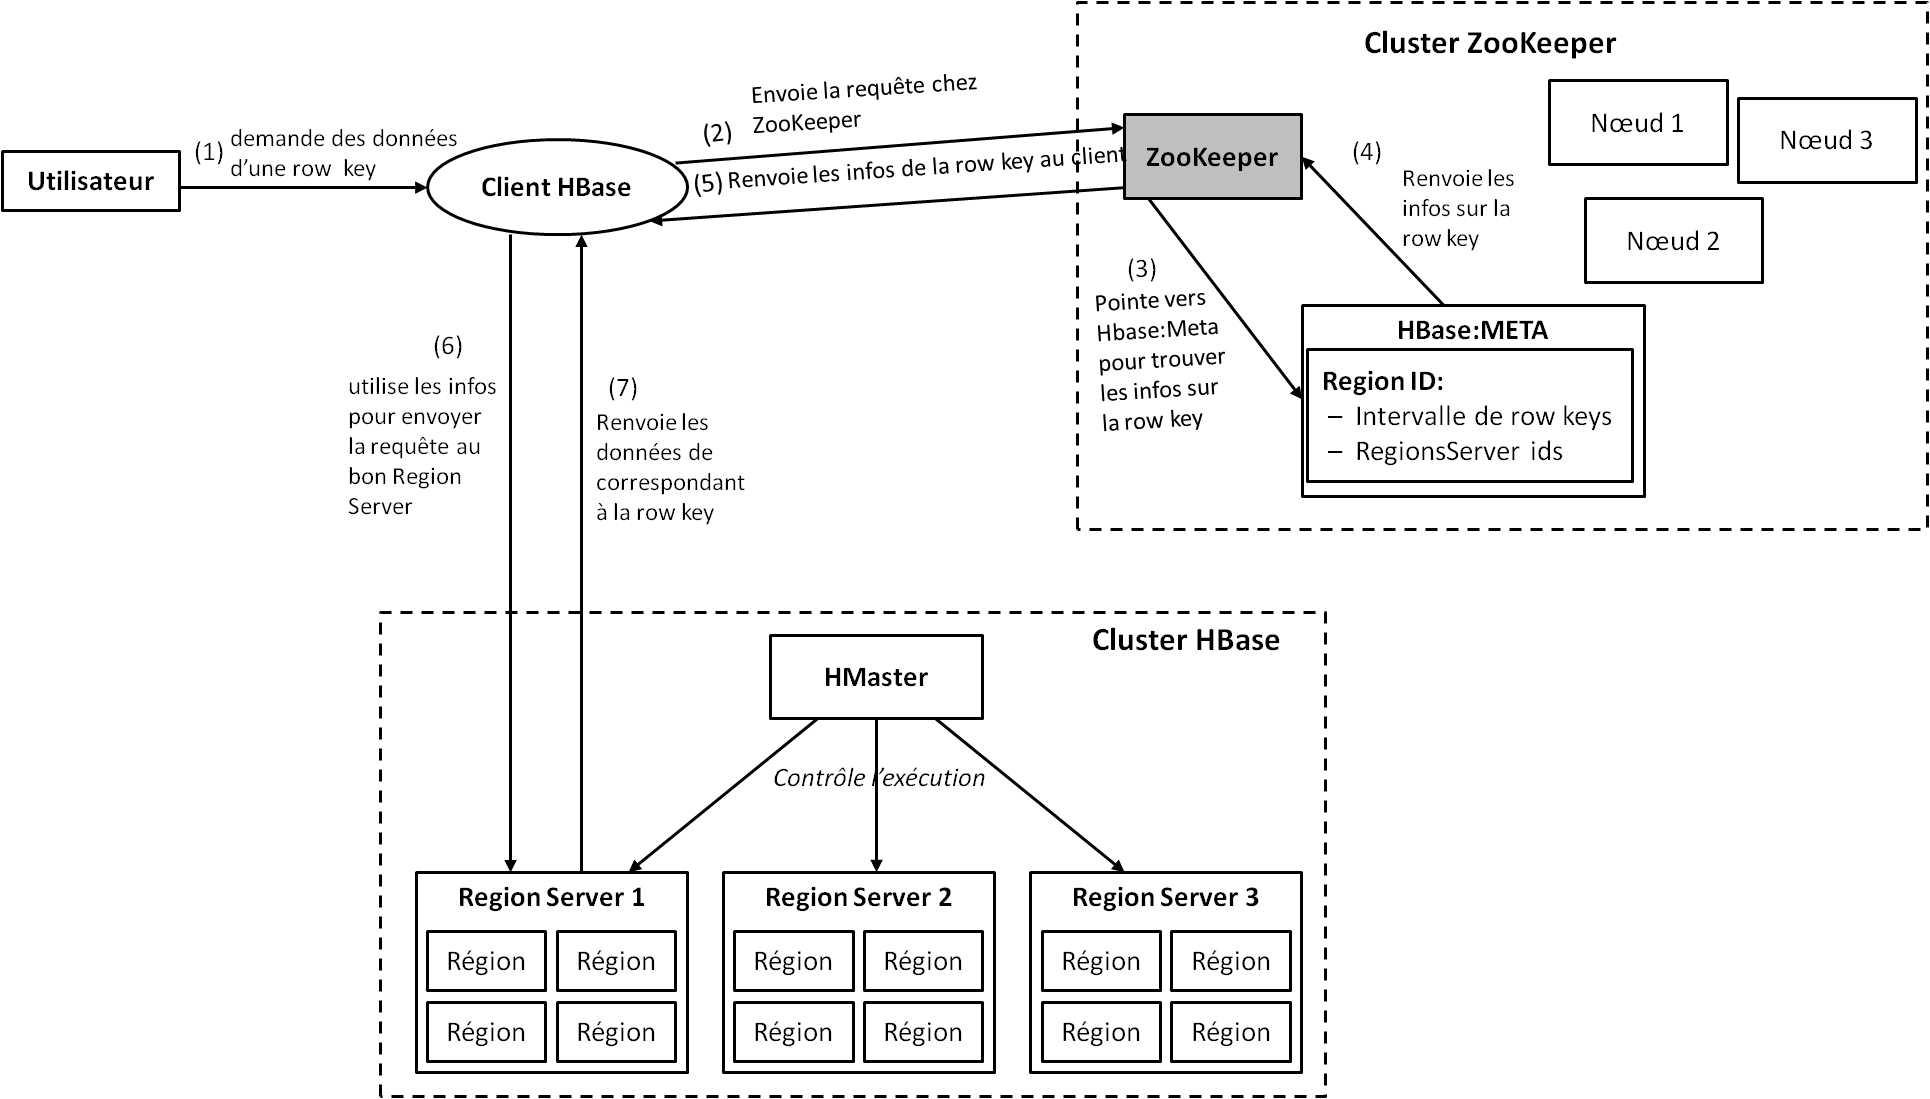
\includegraphics[scale=1]{img/part2/2.4.png}
	\caption{Structuration de donnees sous Cassandra}
\end{figure}

    \newpage
    \section{Le SQL vs le NoSQL:}
Dans un but d'analyse et de comparaison (SQL vs NoSQL), il nous a été demandé de réaliser le modèle E-A relative a notre cas d'étude que nous présenterons ci-dessous ainsi que le modèle relationnel:

\subsection{Le modèle entité association:}


\subsection{Le modèle relationnel:}
Le modèle relationnel est une manière de représenter les relations existantes entre plusieurs informations, et de les ordonner entre elles.
A partir du modèle E-A précédent, on peut faire un passage vers le modèle relationnel en respectant les règles de passage et on obtient le modèle relationnel suivant :

\begin{figure}[h]
	\centering
	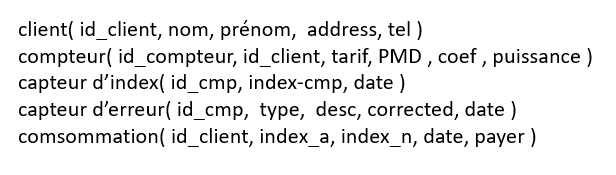
\includegraphics[scale=1]{img/part2/2.6.png}
	\caption{Le modèle relationnel}
\end{figure}

    \newpage
   
    
    \part{Réalisation}
    \chapter{Choix des outils technologiques}
    \section*{Introduction}

Pour la mise en œuvre de notre travail nous avons opté pour l'utilisation des technologies : Hadoop et Hbase pour la mise en place de la base de donnée NoSQL. Tout au long de cette partie nous présenterons les étapes d'installation de ces technologies ainsi que les outils de développement utilisés pour développer un simulateur qui génère des données pour la gestion d'électricité dans le cadre d'un smart grid.

\begin{figure}[h]
	\centering
    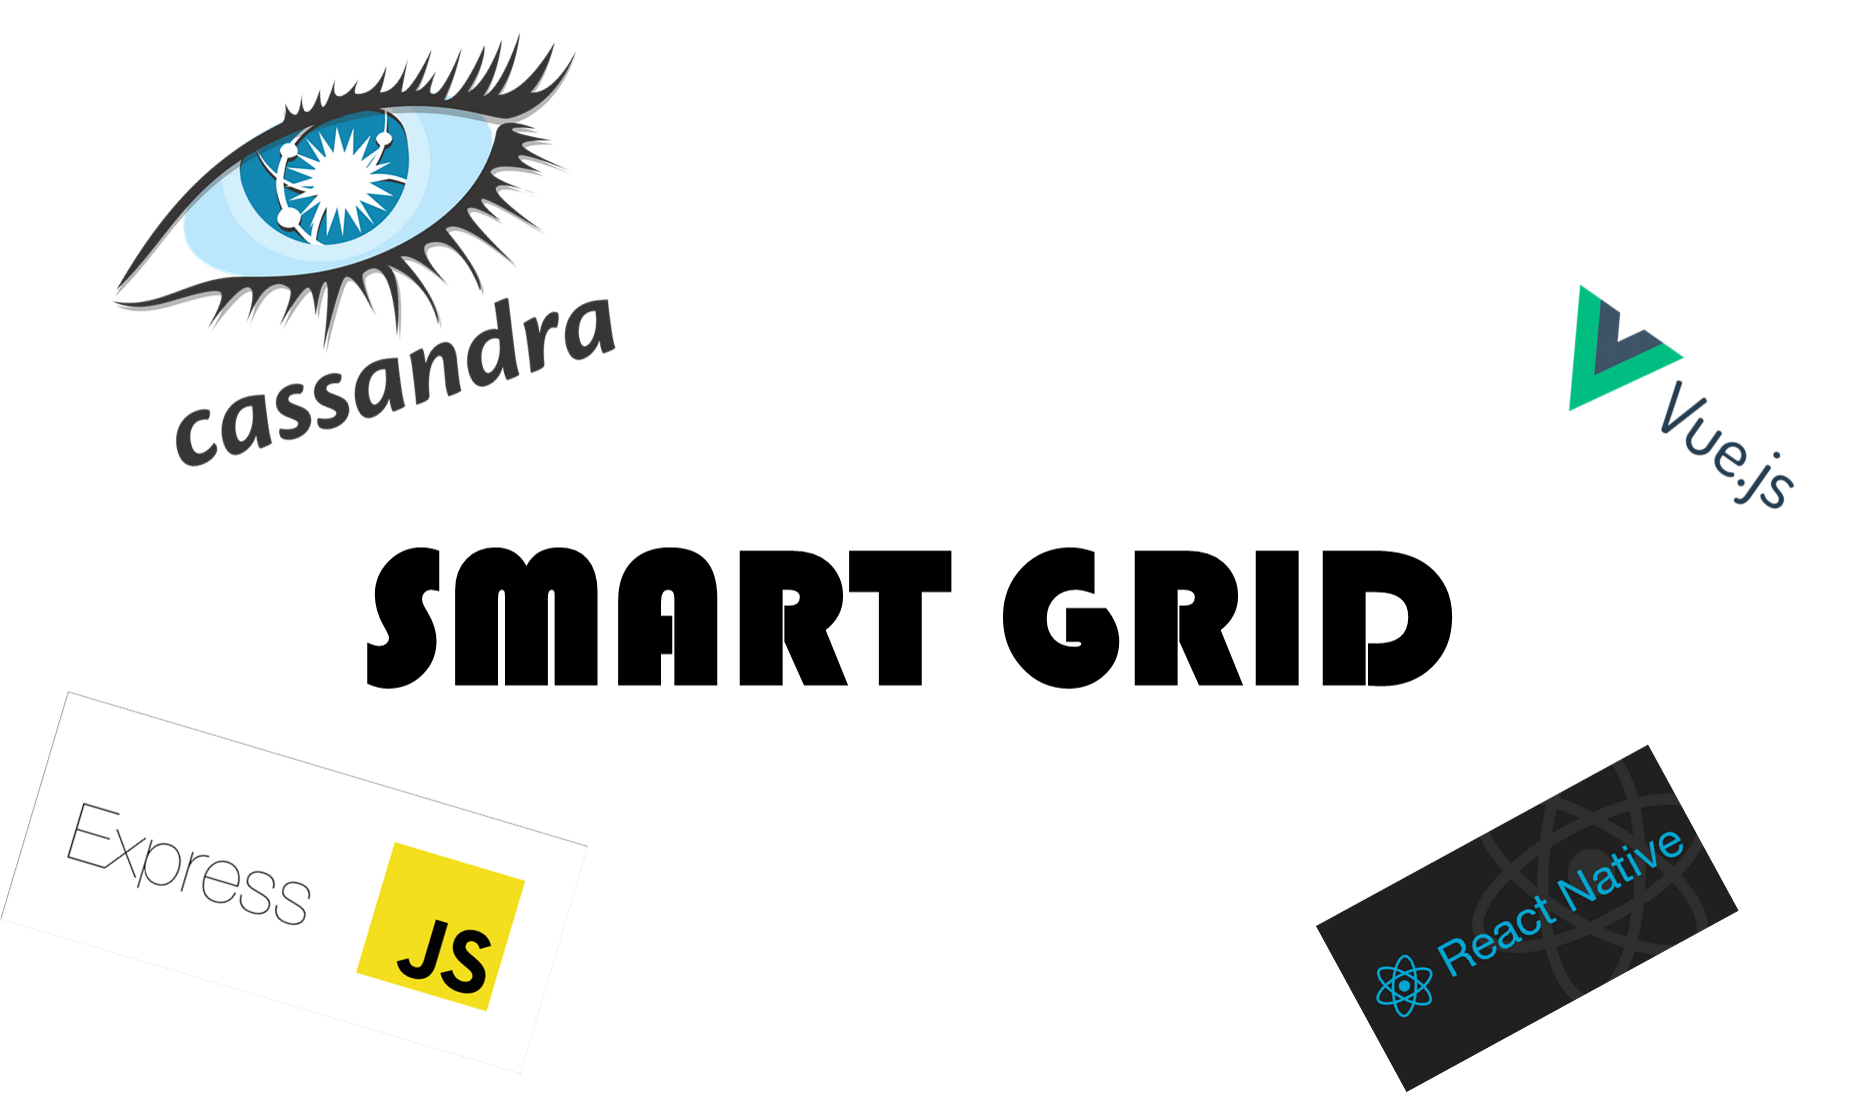
\includegraphics[scale=0.6]{img/part3/1.1}
    \caption{Technologies utilisé}
\end{figure}

    \newpage
    \section{Installation de Cassandra}
    \subsection{Dépendances}
Apache Cassandra nécessite Java 8 pour s'exécuter sur un système Windows. De plus, le shell de ligne de commande Cassandra ( cqlsh ) dépend de Python 2.7 pour fonctionner correctement.

Pour pouvoir installer Cassandra sur Windows, vous devez d'abord :
\begin{enumerate}
\item Téléchargez et installez Java 8 et définissez les variables d'environnement.
\item Téléchargez et installez Python 2.7 et définissez les variables d'environnement.
\end{enumerate}

\begin{figure}[h]
	\centering
    
\includegraphics[scale=0.5]{img/part3/2.1}
    \caption{Java et Python}
\end{figure}

Si vous avez déjà installé ces dépendances, vérifiez votre version de Python et Java. Si vous avez Java 8 et Python 2.7. n'hésitez pas à passer à la troisième section de ce guide.

\newpage
\subsubsection {Étape 01:  Installez Java 8 sur Windows}

\textbf{Télécharger Oracle JDK 8 (Kit de développement Java):}

Le kit de développement Java contient tous les outils et logiciels dont vous avez besoin pour exécuter des applications écrites en Java. C'est un prérequis pour les solutions logicielles telles qu'Apache Cassandra

\begin{enumerate}
\item Visitez la page de téléchargement officielle d'Oracle et téléchargez le progiciel Oracle JDK 8. \href{https://www.oracle.com/java/technologies/javase/javase-jdk8-downloads.html}{lien ici}

\item Faites défiler vers le bas et localisez le lien de téléchargement du kit de développement Java SE 8u251 pour Windows x64. Le téléchargement de Java 8 démarre automatiquement après l'inscription.

\item Une fois le téléchargement terminé, double-cliquez sur le fichier exécutable téléchargé. Sélectionnez Suivant sur l'écran d'installation initiale.

\item La section suivante vous permet de sélectionner des fonctionnalités optionnelles et de définir l'emplacement du dossier d'installation. Acceptez les paramètres par défaut et notez le chemin d'accès complet au dossier d'installation $C:/Java/jdk1.8.0_201$. Une fois que vous êtes prêt à procéder à l'installation, cliquez sur Suivant.

\item Le processus d'installation peut prendre plusieurs minutes. Sélectionnez Fermer une fois le processus terminé.

\end{enumerate}

\textbf{Configurer les variables d'environnement pour Java 8:}

Il est essentiel de configurer les variables d'environnement dans Windows et de définir le chemin correct vers le dossier d'installation de Java 8.
\begin{enumerate}
\item Accédez à Ce PC > Propriétés .
\item Sélectionnez Paramètres système avancés.
\item Cliquez sur le bouton Variables d'environnement… 
\item Sélectionnez Nouveau dans la section Variable système .
\item Accédez à $C:/Java/jdk1.8.0_201$ et sélectionnez OK.
\item Une fois que le chemin correct vers le dossier d'installation JDK 8 a été ajouté à la variable système $JAVA_HOME$ , cliquez sur OK .
\item Vous avez ajouté avec succès la variable système $JAVA_HOME$ avec le chemin JDK 8 correct à la liste des variables. Sélectionnez OK dans la fenêtre principale Variables d'environnement pour terminer le processus.
\end{enumerate}
\newpage
\subsubsection {Étape 2 : installer et configurer Python 2.7 sous Windows:}

Les utilisateurs interagissent avec la base de données Cassandra en utilisant le shell bash cqlsh . Vous devez installer Python 2.7 pour que cqlsh gère correctement les demandes des utilisateurs.

\textbf{Installer Python 2.7 sur Windows}

\begin{enumerate}
\item Visitez la page de téléchargement officielle de Python et sélectionnez le lien de la version Windows x64. \href{https://www.python.org/downloads/release/python-2718/}{lien ici}
\item Définissez si vous souhaitez que Python soit disponible pour tous les utilisateurs de cette machine ou uniquement pour votre compte utilisateur et sélectionnez Suivant .
\item Spécifiez et notez l'emplacement du dossier d'installation de Python. N'hésitez pas à laisser l'emplacement par défaut C:Python27 en cliquant sur Suivant.
\item L'étape suivante vous permet de personnaliser le package d'installation Python. Sélectionnez Suivant pour continuer l'installation en utilisant les paramètres par défaut.
\item Le processus d'installation prend quelques instants. Une fois terminé, sélectionnez Terminer pour terminer le processus d'installation.
\end{enumerate}

\textbf{Modifier la variable d'environnement pour Python 2.7}
\begin{enumerate}
\item Accédez à Ce PC > Propriétés .
\item Sélectionnez l' option Paramètres système avancés .
\item Cliquez sur Variables d'environnement…
\item Double-cliquez sur la variable système Path existante .
\item Sélectionnez Nouveau , puis Parcourir pour localiser rapidement le dossier d'installation de Python. Une fois que vous avez confirmé que le chemin est correct, cliquez sur OK .
\item Ajoutez le chemin Python 2.7 à la variable système Path en sélectionnant OK.
\end{enumerate}
\newpage
\subsubsection {Étape 3 : Téléchargez et configurez Apache Cassandra:}

\textbf{Télécharger et extraire le dossier Cassandra tar.gz}

\begin{enumerate}
\item Visitez la page officielle de téléchargement d'Apache Cassandra et sélectionnez la version que vous préférez télécharger. Actuellement, la dernière version disponible est 3.11.6.\href{https://cassandra.apache.org/_/download.html}{lien ici}
\begin{figure}[h]
	\centering
    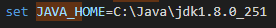
\includegraphics[scale=0.6]{img/part3/2.2}
    \caption{Site de téléchargement de Cassandra}
\end{figure}
\item Cliquez sur le lien de téléchargement miroir suggéré pour démarrer le processus de téléchargement.
\begin{figure}[h]
	\centering
    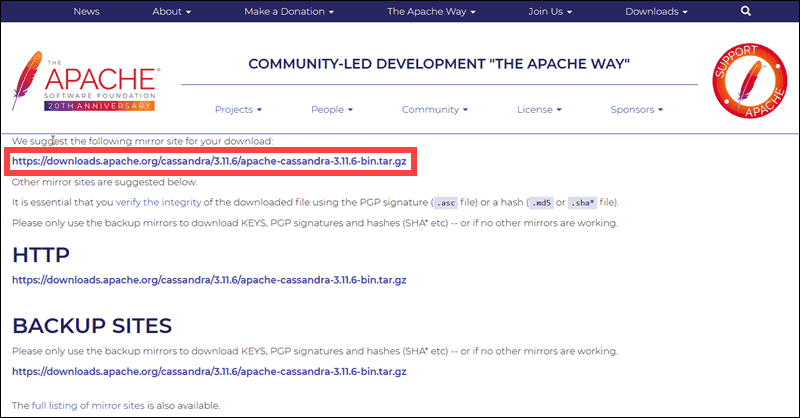
\includegraphics[scale=0.5]{img/part3/2.3}
    \caption{le lien de téléchargement miroir}
\end{figure}
\newpage
\item Décompressez le dossier tar.gz compressé à l'aide d'un outil de compression tel que 7-Zip ou WinZip. Dans cet exemple, le dossier compressé a été décompressé et le contenu placé dans le dossier C:/Cassandra/apache-cassandra-3.11.6.
\begin{figure}[h]
	\centering
    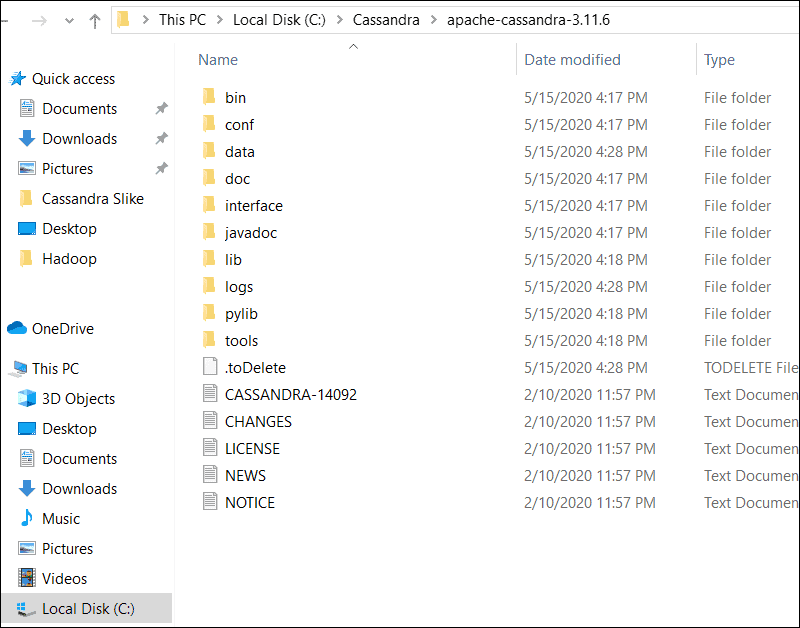
\includegraphics[scale=0.5]{img/part3/2.4}
    \caption{contenu du dossier}
\end{figure}
\end{enumerate}

\textbf{Configurer les variables d'environnement pour Cassandra:}

Configurez les variables d'environnement pour Cassandra afin de permettre à la base de données d'interagir avec d'autres applications et de fonctionner sous Windows.

\begin{enumerate}
\item Accédez à Ce PC > Propriétés.
\item Accédez à Paramètres système avancés .
\item Cliquez sur le bouton Variables d'environnement… .
\item Ajoutez une toute nouvelle entrée en sélectionnant l' option Nouveau .
\item Tapez $CASSANDRA_HOME$ pour Nom de la variable , puis pour la colonne Valeur de la variable , sélectionnez l'emplacement du  dossier Apache Cassandra décompressé.

Sur la base des étapes précédentes, l'emplacement est C:/Cassandra/apache-cassandra-3.11.6. Une fois que vous avez confirmé que l'emplacement est correct, cliquez sur OK.
\item Double-cliquez sur la variable Chemin .
\item Sélectionnez Nouveau puis Parcourir . Dans ce cas, vous devez ajouter le chemin complet du  dossier bin situé dans le dossier Apache Cassandra, C:/Cassandra/apache-cassandra-3.11.6bin .
\item Appuyez sur le bouton OK , puis à nouveau sur OK pour enregistrer les variables modifiées.
\end{enumerate}
\newpage
\subsubsection {Étape 3 : Démarrez Cassandra à partir de Windows CMD:}
Accédez au dossier Cassandra bin. Démarrez l'invite de commande Windows directement à partir du dossier bin en tapant cmd dans la barre d'adresse et en appuyant sur Entrée .

\begin{figure}[h]
	\centering
    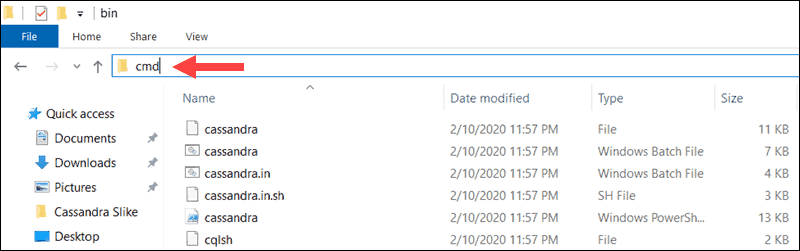
\includegraphics[scale=0.6]{img/part3/2.5}
    \caption{dossier Cassandra bin}
\end{figure}

Tapez la commande suivante pour démarrer le serveur Cassandra :

\begin{center}
$cassandra$
\end{center}

Le système démarre le serveur Cassandra.

\begin{figure}[h]
	\centering
    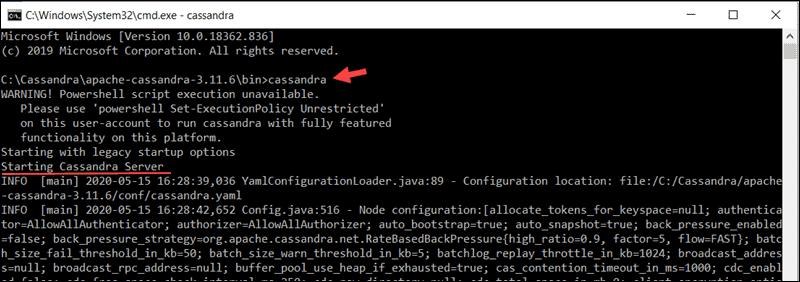
\includegraphics[scale=0.6]{img/part3/2.6}
    \caption{le serveur Cassandra}
\end{figure}

Ne fermez pas la session cmd en cours.
\newpage
\subsubsection {Étape 5 : Accédez à Cassandra cqlsh à partir de Windows CMD:}

Pendant que l'invite de commande initiale est toujours en cours d'exécution, ouvrez une nouvelle invite de ligne de commande à partir du même dossier bin. Saisissez la commande suivante pour accéder au shell bash Cassandra cqlsh :

\begin{center}
$cqlsh$
\end{center}
Vous avez maintenant accès au shell Cassandra et pouvez procéder à l'émission de commandes de base de données de base sur votre serveur Cassandra.

\begin{figure}[h]
	\centering
    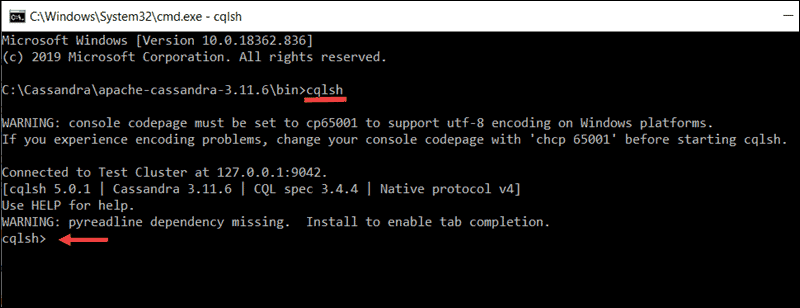
\includegraphics[scale=0.6]{img/part3/2.7}
    \caption{shell Cassandra}
\end{figure}
    \newpage
    \section{Langages et outils de développement}
Pour développer notre propre simulateur on utilise les outils et les langages de programmation suivant :

\subsection{Javascript}
JavaScript est un langage de programmation qui permet d’implémenter des mécanismes complexes sur une page web. À chaque fois qu’une page web fait plus que simplement afficher du contenu statique — afficher du contenu mis à jour à des temps déterminés, des cartes interactives, des animations 2D/3D, des menus vidéo défilants, etc... 
\\JavaScript a de bonnes chances d’être impliqué. C’est la troisième couche des technologies standards du web, les deux premières (HTML et CSS, Les trois couches se superposent naturellement. 
\begin{figure}[h]
	\centering
    
\includegraphics[scale=0.1]{img/part3/4.1}
    \caption{Logo JavaScript}
\end{figure}

\subsection{vue}
Vue.JS, ou simplement Vue, est un framework progressif pour les interfaces utilisateur pour les apps et sites JavaScript. Il s’agit d’un des frameworks front-end JS les plus populaires. On le compare souvent à React, Angular, Ember, etc. Par leur approche et leur ressemblance, Vue et React partagent de nombreux points communs. Le framework apparaît à l’été 2013. Il est développé par Evan You. Peu à peu, Vue va faire parler de lui et s’imposer chez les développeurs JS.
\begin{figure}[h]
	\centering
    
\includegraphics[scale=0.3]{img/part3/4.2}
    \caption{Logo VueJs}
\end{figure}

\newpage
\subsection{nodes}
NodeJS est un outil libre codé en Javascript et orientée pour des applications en réseau. Si vous êtes sur cette page, c’est certainement parce que vous voulez avoir des explications plus détaillées sur NodeJS. Cet outil JavaScript est devenu célèbre dans l’univers du développement web depuis quelques années. D’ailleurs, il est très apprécié des géants du web comme Netflix, PayPal, LinkedIn, Uber, la NASA, etc. Cet article basé sur la définition de NodeJS se donne pour rôle de vous faire découvrir de long en large cette technologie. Vous y trouverez également tous les avantages liés à son utilisation.
\begin{figure}[h]
	\centering
    
\includegraphics[scale=0.4]{img/part3/4.3}
    \caption{Logo NodeJs}
\end{figure}

\subsection{express js}
ExpressJS est un framework qui se veut minimaliste. Très léger, il apporte peu de surcouches pour garder des performances optimales et une exécution rapide. Express ne fournit que des fonctionnalités d’application web (et mobile) fondamentales, mais celles-ci sont extrêmement robustes et ne prennent pas le dessus sur les fonctionnalités natives de NodeJS. 
\begin{figure}[h]
	\centering
    
\includegraphics[scale=0.1]{img/part3/4.4}
    \caption{Logo ExpressJs}
\end{figure}
    
    




     
    \bibliographystyle{plain}
	\bibliography{bibl}
  
\end{document}